\immediate\write18{makeindex \jobname.nlo -s nomencl.ist -o \jobname.nls}

\documentclass[conference]{IEEEtran}
%\IEEEoverridecommandlockouts
% The preceding line is only needed to identify funding in the first footnote. If that is unneeded, please comment it out.
\usepackage{cite}
\usepackage{amsmath,amssymb,amsfonts}
\usepackage{algorithmic}
\usepackage{graphicx}
\usepackage{textcomp}
\usepackage{tikz}
\usetikzlibrary{arrows}
\usepackage{verbatim}
\usepackage{graphicx}
\usepackage{subfig}
\usepackage{dblfloatfix}
\usepackage{blkarray}
\usepackage{fancyhdr}
\usetikzlibrary{automata,positioning}
\usetikzlibrary{fit}
\pagestyle{empty}
\usepackage{xcolor}
 \usepackage{nopageno}
 \usepackage{xcolor,graphicx}
\usepackage[belowskip=-10pt,aboveskip=0pt]{caption}
\usepackage{hyperref}
%\setlength{\intextsep}{10pt plus 2pt minus 2pt}
\usepackage{imakeidx}
\usepackage{tikz} % the tikz package  
\usetikzlibrary{shapes.geometric, arrows}   
\makeindex

\usepackage{nomencl}
\makenomenclature

\newcommand\coolover[2]{\mathrlap{\smash{\overbrace{\phantom{%
\begin{matrix} #2 \end{matrix}}}^{\mbox{$#1$}}}}#2}

\def\BibTeX{{\rm B\kern-.05em{\sc i\kern-.025em b}\kern-.08em
T\kern-.1667em\lower.7ex\hbox{E}\kern-.125emX}}
\usepackage{microtype} % Load this package to obtain a fine composition.


\IEEEpubid{
}

\newcommand{\conftitle}{}

\usepackage{fancyhdr}
\chead{\conftitle}
\cfoot{\thepage}

% style for the first page only
\fancypagestyle{pageStyleOne}{%
    \fancyhf{}
\renewcommand{\headrulewidth}{0pt}
    \fancyhead[C]{\conftitle}
%   \fancyfoot[C]{\thepage}    % do you want page number on the first page?
    \fancyfoot[L]{}
}

\makeatletter
\makeatother

%\thispagestyle{empty}

%% This code creates the groups
% -----------------------------------------
\usepackage{etoolbox}
\renewcommand\nomgroup[1]{%
  \item[\bfseries
  \ifstrequal{#1}{P}{Data Representations}{%
  \ifstrequal{#1}{N}{Number sets}{%
  \ifstrequal{#1}{O}{Abbreviations}{}}}%
]}
% -

\setlength{\nomlabelwidth}{3.5cm}
%\usepackage{enumitem}
%\newlist{steps}{enumerate}{1}
%setlist[steps, 1]{label = Step \arabic*:}

\begin{document}

\title{Associative memory based SLFM method for estimating suspect SCADA data -NR Grid case study\\
%{\footnotesize \textsuperscript{*}Note: Sub-titles are not captured in Xplore and should not be used}
%\thanks{Identify applicable funding agency here. If none, delete this.}
}
\author{\IEEEauthorblockN{\textit{S. Naresh Ram} }
\IEEEauthorblockA{\textit{POSOCO}\\
New Delhi, India \\
naresh.ram@posoco.in}

\and
\IEEEauthorblockN{\textit{Sukumar Mishra} }
\IEEEauthorblockA{\textit{IIT Delhi}\\
New Delhi, India \\
sukumar@ee.iitd.ac.in}

\and
\IEEEauthorblockN{\textit{S.Lakra} }
\IEEEauthorblockA{\textit{POSOCO}\\
New Delhi, India \\
somara.lakra@posoco.in }
\and
\IEEEauthorblockN{\textit{N.Nallarasan} }
\IEEEauthorblockA{\textit{POSOCO}\\
New Delhi, India \\
nallarasan@posoco.in }
}

\maketitle
\thispagestyle{pageStyleOne}


\begin{abstract}
Power System operator decisions depend on available real-time measurement through Supervisory Control and Data Acquisition (SCADA) system . Whereas, under external disturbances, failure in Fiber Optic (FO) cable, sensors etc causes displaying suspect/erroneous data to the operator. To ensure reliable operation of power grid under such cases proposes an interpretable data-driven Soft Lookup False data Matching (SLFM) through Dynamic Time Warping (DTW) model based on associative memory technique for estimating complex pattern of missing/suspect SCADA data values. Numerical experiments conducted on State X of the Northern region of the Indian Grid with real-time data (SCADA and Meter) of PoC feeders for four different cases and compared the results with (LSTM-Autoencoder) model. The experimental results demonstrate the performance of the proposed model\\
\end{abstract}
\begin{IEEEkeywords}
Autoencoder,Dynamic Time warping, Energy Management system, False Data, India,Long Short Term Memory, SCADA, 
\end{IEEEkeywords} 
\mbox{}
\nomenclature[P]{\(z^m_{j,t} \in {M^{nxd}} \  \)}{\ \ \ Meter(True) data}
\nomenclature[P]{\(z^s_{j,t} \in {S^{nxd}} \  \)}{\ \ \    Measurement(SCADA) data}
\nomenclature[P]{\(z^{sc}_{j,t} \in {C^{kxd}} \  \)}{\ \ \ Corrupted Measurement data}
\nomenclature[P]{\({D_S} \)}{\ \ \ Database of Measurement data}
\nomenclature[P]{\({D_M} \)}{\ \ \ Database of Meter data}
\nomenclature[P]{\(A,B \dots N \ \in P_g\)}{\ \ \ PoC points of Grid-Stae X}
\nomenclature[P]{\(Ax,Bx \dots Nx \ \in P_x\)}{\ \ \ P0C points of State X-Grid}
\nomenclature[P]{\(\phi \colon D_S\mapsto D_M\)}{\ \ \ Mapping function}
\nomenclature[N]{\(\mathbb{R}\)}{\ \ \ Real Numbers}
\nomenclature[O]{\(PoC\)}{\ \ \ Point of Connection}
\nomenclature[O]{\(GAN\)}{\ \ \ Generative Adversarial Network}
\nomenclature[O]{\(LSTM\)}{\ \ \ ,Long Short Term Memory}
\printnomenclature

\section{Introduction}
Power is among the most critical components of infrastructure, crucial for the economic growth and welfare of nations. The existence and development of adequate infrastructure is essential for sustained growth of the Indian economy.\\
 
India's power sector is one of the most diversified in the world,  consisting more than 600 generating stations, more than 30 transmission licensees , 70 odd distribution licensees , 2 power exchanges, 40 odd trading licensees, National level Load dispatchers at the center, Regional level load dispatchers in  each of the five regions and State level load dispatchers in each of the 28 States. The total installed generation capacity is 383 GW (as of April 2021), out of which 54\% is from coal, about 13\% Hydro, 24\% Renewable, 7\% Gas, and 2\% Nuclear.\\

\begin{comment}
Transferring 180GW (Max as on May 2021) of power  through 1,00,000+ ckt Kms to 138 crore people by maintaining such narrow frequency band (49.95 to 50.05 ) is almost impossible without market involvement. Indian Electricity market  stood on four different pillars i.e  Scheduling and Dispatch, Mechanism for handling imbalances, Congestion management and Ancillary Services.\\

Out of many available mechanisms(Real time market, Short time open access, Day ahead market) for handling imbalances, Central Electric Regulatory Commission of India has come out with a Deviation Settlement Mechanism Regulations \cite{b1} to improve grid discipline by way of proper forecasting and scheduling, so that the actual deviation is minimized.   The Deviation price vector is linked to frequency and average DAM (Day Ahead Market) prices, to give proper commercial signal to all market participants.\\

Under Fourth paradigm, industrial revolution took place with the advances in machine learning techniques several innovations took place  in detection and estimation problems e.g. Reconstructing old images through autoencoder, inferring the true distribution through Generating Adversarial Network, Temporal correlation in Load forecasting using  LSTM etc.Data driven model plays a crucial role in estimating or detecting such attacks  In \cite{b3} the authors proposed (GMM) based model to classify  normal operating conditions to that of intrusion states.\\

\end{comment}
Recently , an event (depicted in figure 1) occurred in Northern Region of Indian Grid, due to inclement weather conditions in the state utiity network (X), its drawl deviated from schedule to a large extent. The state LDC took corrective action to control its under drawl from grid of quantum 300MW only (based on available SCADA data and system operator's experience), whereas, its actual deviation was around 800MW.\\

\begin{figure}
\includegraphics[width=1\linewidth]{Fig1.PNG}
\caption{State X drawl Actual vs Measure vs Schedule}
\end{figure}
However, the state X was unaware of its actual load during that period due to suspect SCADA measurements, which led to load generation imbalance of around 800MW. To avoid such cases, there is a need for the tool which estimates the individual feeder data even under suspect measurement and topology.
\subsection{Related Works}
The missing data imputation can be done through a)Naive method, which involves comparing the erroneous/suspect data with previous or average of historical data. If the difference is above the threshold, then the corrupted data be replaced with historical average values. This method failed whenever missing occurs for a longer period. b) Multivariate time series \cite {b7} \cite{b8} \cite{b13},electrical loads typical random and volatile, which makes missing imputation is difficult with classic multivariate linear systems. c) Low rank approximation \cite{b16} models captures the temporal relations but fails in time dependencies. Moreover, not every big data be represented as low rank approx.\\

On the other hand, estimating suspected data comes under the purview of data driven models of defending False Data Injection Attacks(FDIA) \cite{b2} , Matrix Completion \cite{b3} and Load Forecasting with missing data\cite{b4} \cite{b9}.In all the areas of problem, applying Machine learning based algorithm of LSTM/Recurrent neural network with Auto encoder achieved State Of The Art results. \\

Here LSTM layer helps in transforming non stationary data to stationary and makes the model learns both spatial and temporal relations between them. Hence, LSTM based models better than classic models \cite{b6}. However, the problem of estimating the uncertainty in time series data remains an open question.\\

\subsection{Main contributions of the paper}
Due to inexplicable, the efficacy of machine learning for time series prediction has been questioned for its guarantee and robustness. We proposed a  method(SLFM) based on associative memory search technique, which is inspired from mainly \cite{b11} \& \cite{b12}, that has high interpret ability and guarantee in convergence to unique point. Moreover, this paper highlights the use of Dynamic  Time Warping (DTW) method for time series matching as similarity measure for perfect recall.\\

\section{Soft Lookup based False data Matching (SLFM) model for estimating true data from corrupted measurement data}

\subsection{Problem formulation }

Generalized modeling for predicting/estimating the true data from the suspected measured time series data of length $d$ through the logical grouping of temporal information of feeders data ($j=1:n$) of state X i.e, let the K feeders of  $P_g$ and its corresponding other end in $P_x$ has corrupted measurement data be denoted as  $C^{kxd}$  and $C$ $\subset S \subset D_S$. For an instant T, the true measurement ($ z^{*{sc}}_{j:k,T}$) of $k$ suspected feeders data ($ z^{{sc}}_{j:k,T}$) be estimated through generalized model as shown below.i.e finding a perfect matching pair to suspect data point from mapping set $\phi$ of databases through a loss function {h}.

\begin{align*} 
 z^{*{sc}}_{j:k,T} = \underset{Z \in \psi} {\text{inf}} h( z^{sc}_{j:k,T},Z) \tag{1} \text{ here h is loss function}
\end{align*}

\begin{figure}
\includegraphics[width=1\linewidth]{Connect_X.PNG}
\caption{State X poc feeders connectivity with Grid poc}
\end{figure}
In General, under no external influences the flow pattern remains similar to very previous day pattern, If there exists any forced disturbances like fiber optical failure, weather disturbance, cyber attack etc  their signature is unique to classify. With the domain knowledge, the experience operator able to bypass few of such cases and makes the grid secure and reliable. \\

Inspiring from human intellect, a model proposed for triggering proper recall through database of stored meter data ($D_M$) and Measurement data ($D_S$) with partial/noisy measurement ($C$) using associative memory technique.\\

\subsection{DTW- a perfect measure for time series data}

In the domain of sequence data analysis( time series ), both Minkowski and Mahalanobis distances fail to reveal the true similarity between two targets. Dynamic Time Warping (DTW)  \cite{b17} has been proposed as an attractive alternative.\\
Hence DTW is widely used for similarity measure between time series data. Moreover,DTW provides more meaningful discrepancy measurements between two signals than other distance measures \cite{b18}. \\
\begin{align*}
DTW(z^s,z^{sc})=\underset{\pi} {\text{min}}{\sum^{n}_{(i,j) \in \pi}\sqrt{||z^s_{i}-{z^{sc}_{j}}||}} \tag{2}\\
 \text{ where $\pi$ is  time series  align paths  [$\pi_1 \dots \pi_p$] }
\end{align*}
 The above objective function be solved through dynamic programming as depicted in \cite{b10}
\begin{align*}
& \zeta_{i,k}=||z^s_{j,i}-{z^{sc}_{j,k}}|| + \text{min }\{\zeta_{i-1,k},\zeta_{i,k-1},\zeta_{i-1,k-1}\}\\
 & DTW(z^s_{i,j},z^{sc}_{k,j})=\sqrt{\zeta_{i,k}}\\
\end{align*}

\subsection{Soft Lookup False data Matching model- recall method}
We now introduce new SLFM method for recalling the true measurement $z^{{m}}_{j} \subset M$ through a query (corrupt data ) $(z^{sc}_j)\subset C$.\\

Proposed method mainly consists of two steps.
\begin{itemize}
\item  Recursively multiplying(associatively) the probability distribution of similarity function ($ S(D_{S},{z^{sc}_{j}})$) with data base ($D_S$) (memory) to get nearest match of suspect measurement within database.\\
\item  Choosing the corresponding meter data from $D_M$ for the converged signature of corrupted data through the mapping table ($\phi$) between $D_S \ \& \ D_M$.
\end{itemize}
\begin{comment}
\begin{align*} 
 z^{m}_j = \phi \big \{D_M,\underset{\zeta \sim D_{S} }{\text{argmin}} \big \{ DTW( \zeta,z^{sc}_{k,j})\big\} \big \}
\end{align*}
\end{comment}
The probability distribution of similarity points over Database ($D_S$) be achieved through $softmax()$ function.\\

Moreover, we claim that under well separated/ independent stored time series data, there exists a unique retrieval point through SLFM method for the suspected Measurement data point and the proof of such claim in Appendix 1.
\begin{align*}
 z^{sc}_{j,t }& =D_{S}^T.{( \frac{exp(S(D_{S},{z^{sc}_{j,t-1}}))}{\sum_k exp(S(D_{Sk} ,{z^{sc}_{j:n,t-1}}))} )}\\ \\
& =D_{S}^T.{(softmax(S(D_S,{z^{sc}_{j,{t-1}}})))} \tag{3} \\ \\
& \sim \text{converges to  $z^{s}_{j}\in S \subset D_S$ } \\
& \text{Here } S(D_{S},{z^{sc}_{j}})  = \sum_{i,k}{DTW({z^s_{i,j},z^{sc}_{k,j}})}
\end{align*}
Now recalling the true meter data for the respective SCADA measurement through mapping table $\phi$.
\begin{align}
z^{{m}}_{j} &= \phi(D_{M},z^{s}_{j}) \ \text {where  $\phi \colon D_S\mapsto D_M$ $\bf{one\ to\ one}$} \tag{4} 
\end{align}
Here $z^{{*m}}_{j:k} \subset z^{{m}}_{j:n}$ is the perfect recall for the corresponding corrupted data $z^{sc}_{j:k}$.\\

\section{proposed model (SLFM) flow chart}

The flow chart of the process model is shown above, here, the loop runs until the threshold $\epsilon$ reaches. However, for well separated case, not more than two loops required for attaining convergence. Here, $true$ data means the true meter data of the suspected feeder data.\\

 In our case, the true validated meter data generally available after 7 days, hence the log for the error be maintained to update the data base. If the estimated and error below the threshold (our case, we took 100) then no need for any change/modify the databases ($D_M \ \& \ D_S$)

\tikzstyle{decision} = [diamond, draw, fill=orange!80,   
    text width=5.0em, text centered, node distance=3.1cm,]   
    \tikzstyle{document} = [rectangle, draw, fill=blue!30,   
    text width=4.7em, text centered, node distance=2.5cm,]   
   \tikzstyle{block1} = [rectangle, draw, fill=green!50,  %here, we have chosen another block for the different color  
    text width=5.5em, text centered, rounded corners, node distance= 3cm, minimum height=3em] % you can create as many different shapes to make your diagram more creative and attractive, depending on the requirements  
 \tikzstyle{block2} = [rectangle, draw, fill=green!50,  
    text width=4.0em, text centered,rounded corners, node distance= 3.0cm]
\tikzstyle{block} = [rectangle, draw, fill=yellow!50,   
    text width=4.5em, text centered, rounded corners, node distance=2.25cm, minimum height=4em]  
\tikzstyle{line} = [draw, -latex']  
\tikzstyle{cloud} = [draw, ellipse,text width= 2.9em, fill=red!50, node distance=3cm, minimum height=3em]  
\tikzstyle{cloud1} = [draw, ellipse,text width= 3.1em, fill=red!20, node distance=3cm, minimum height=3em]  
  
\tikzstyle{ioi} = [trapezium, draw, trapezium right angle=120,rounded corners, fill=blue!60, node distance=2.8cm, minimum height=2.7em]  
 \tikzstyle{io} = [trapezium, draw, trapezium right angle=110,rounded corners, fill=red!20, node distance=1.9cm, minimum height=2.9em]   % the draw command here is used to draw the boundary of mentioned shape.  
\begin{tikzpicture}[node distance = 1.8cm, auto] % the command node distance is important as it determines the space or the length of the arrow between different blocks.  
    % the command given below are the place of nodes  
    \node [cloud] (init) {Start};  
    \node [io, below of=init](A){$C,M,S,D_M,D_S,\epsilon,\delta,$};  
    \node [block, below of = A](D){$z^{sc}_{j,t}$};  
    \node [decision, below of = D](E){$||z_{j,t}-z_{j,t-1}|| \le \epsilon$};    
    \node [block2, right of = E](H){$softmax$};  
    \node [block1, below of = H](I){$S(D_S,z^{sc}_{j,t-1})$};  
\node [cloud1, below of = I](O){$D_S$};  
    \node [cloud1, left of = D](J){$D_M$};  
    \node [block1, left of = E](K){$\phi(D_m,z^s_j)$};
 \node [decision, below of = K](N){$||z^m_j-True|| \le\delta$};  
 \node [block1, right of = N](F){Update $D_M \& D_S$};
\node [cloud, below of = F](G){STOP};  
    \path [line] (init) -- (A);   
    \path [line] (A) -- (D);  
    \path [line] (D) -- (E);   
    \path [line] (F) -- (G);   
    \path [line] (E) -- node [near start] {No} (H);   
     \path [line] (E) -- (K);   
    \path [line] (I) -- (H);   
    \path [line] (J) -- (K);   
\path [line] (O) -- (I);   
\path [line] (K) -- (N); 
\path [line] (N) --node [near start] {No} (F); 
 \path [line] (N) |- (G.west);   
    \path [line, dashed] (H) |- (D); % the dashed command is used to create the dashed line   
\end{tikzpicture}  
\section{Results}
\subsection{Data setup and analysis}
State x net drawl is being calculated from the interconnected 26 nos of feeders, the drawl details have been shown in fig \ref{hist2}. For estimating the corrupt data using LSTM and SLFM, all 24nos of feeder's drawl (MW) meter and as well as its respective MW values in SCADA was collected for 3 months of 15-minute interval. The collected data clustered into 40 different groups as per their DTW distances( between Measurement and Meter data).\\

From the heat plot of meter data in fig \ref{hist1}, noticed that all the feeders data are independent of each other. Whereas, dependencies/high correlation observed in between parallel feeders only i.e (feeders 7,8,9,$\&$10). Moreover, from the histogram plot of fig \ref{hist1}, understood that the feeders of 2,12,13,24,25 are almost ideally loaded most of the time.\\

Further, with SCADA (Measurement data) plots fig 4, noticed that feeder 16 data has zero value throughout the collected period. From fig \ref{per3}, on an average 10 $\%$ of SCADA data being corrupted/ stuck at a particular value.\\

All the simulations and test cases are done on python, for the LSTM autoencoder we used Pytorch model run on NVIDIA GeForce GTX 1050Ti and having Ram 8GM of windows 10 PC.\\

\begin{table}[h!]
  \begin{center}
    \caption{Cases of faulty measurement data } 

    \label{tab:table2}
      
       \begin{tabular}{l|c|r} % <-- Alignments: 1st column left, 2nd middle and 3rd right, with vertical lines in between 
      \textbf{CaseNos} & \textbf{Conditions} & \textbf{Suspect feeders}\\ \\
      \hline
      1 & Parallel feeder data suspect & 18, 19\\
      2 & False data injection  & 8,9,10,11\\
      3 & Unknown weather disturbance & 22,23,25,26\\
      4 & Normal operating condition & 16\\
    \end{tabular}
  \end{center}
\end{table}

We selected four different cases as shown in Table 1, We compared the results of proposed model (SLFM) with LSTM auto encoder in every case  and the results discussed comprehensively.
\begin{figure}[!ht]
\includegraphics[width=1\linewidth]{new_mm.PNG}
\caption{Meter State X feeder's drawl Heat plot and histogram }
\label{hist1}
\end{figure}
\begin{figure}[!ht]
\includegraphics[width=1\linewidth]{nn_ms.PNG}
\caption{SCADA State X feeder's drawl Heat plot and histogram }
\label{hist2}
\end{figure}
\begin{figure}
\includegraphics[width=1\linewidth]{msd_modes.PNG}
\caption{Percentage of Measured feeder's data stuck at specific value of State X}
\label{per3}
\end{figure}


\subsection{Testing results and discussions}

We conducted the tests on the above depcted four cases and the results are shown, for case1 , the proposed method is robust to suspect/stuck at any particular value of any feeder data, the estimated through SLFM is the smart lookup to nearest DTW distance. The distance found to be 19, retrieved the corresponding data of nearest distance and the error wrt to true is almost zero. Whereas it's a known fact, the decisions/ estimated with ML techniques are sensitive to noise/disturbance, hence the error incurred with LSTM is more than anticipated which is shown in fig \ref {case1}.\\

\begin{figure}[!ht]
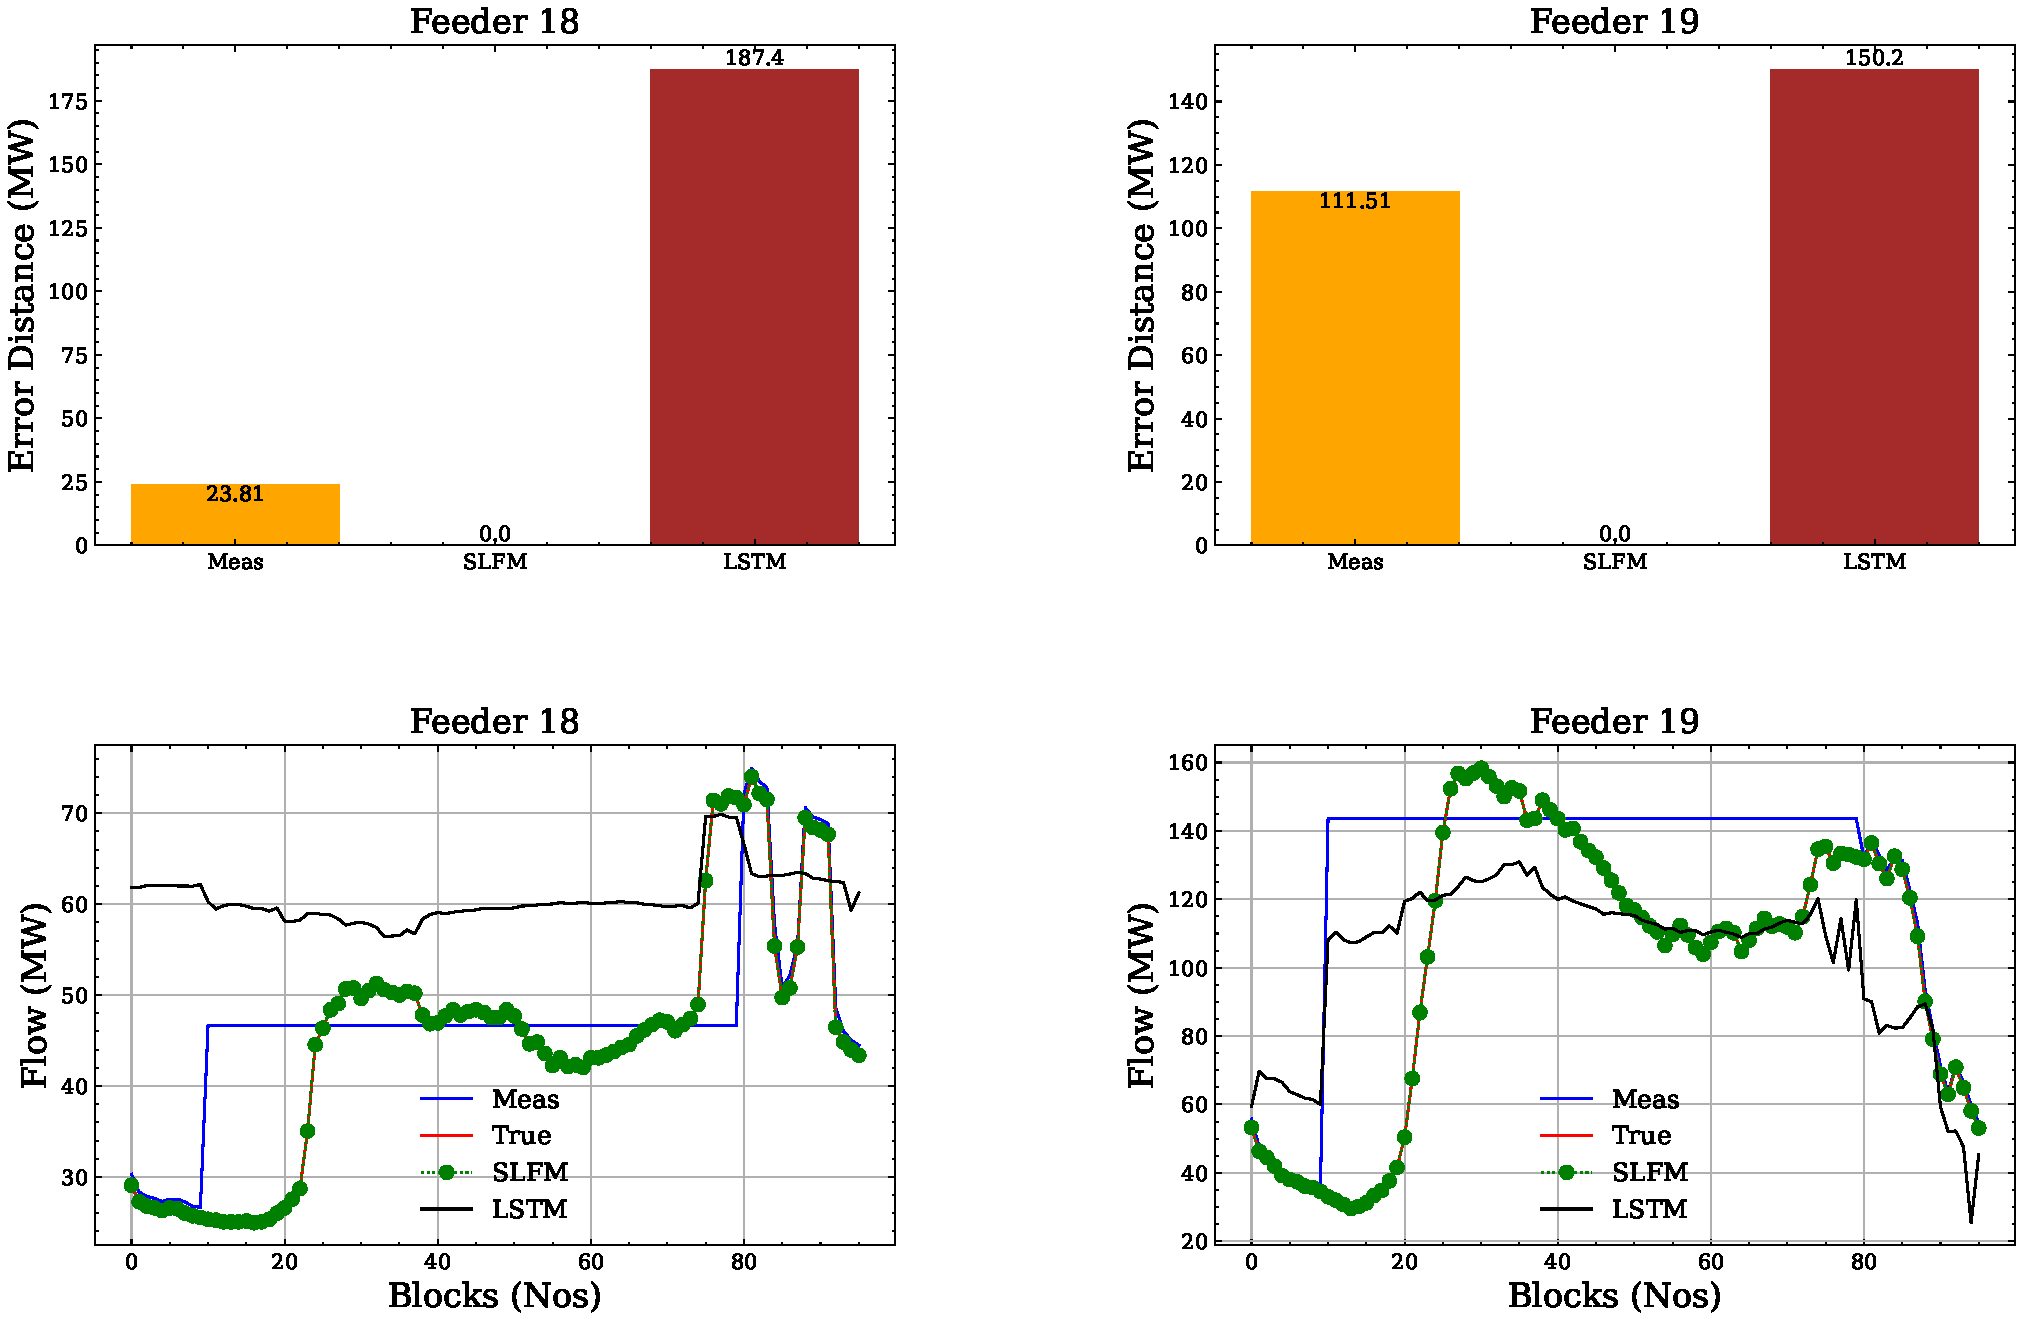
\includegraphics[width=1\linewidth]{Test_results11.pdf}
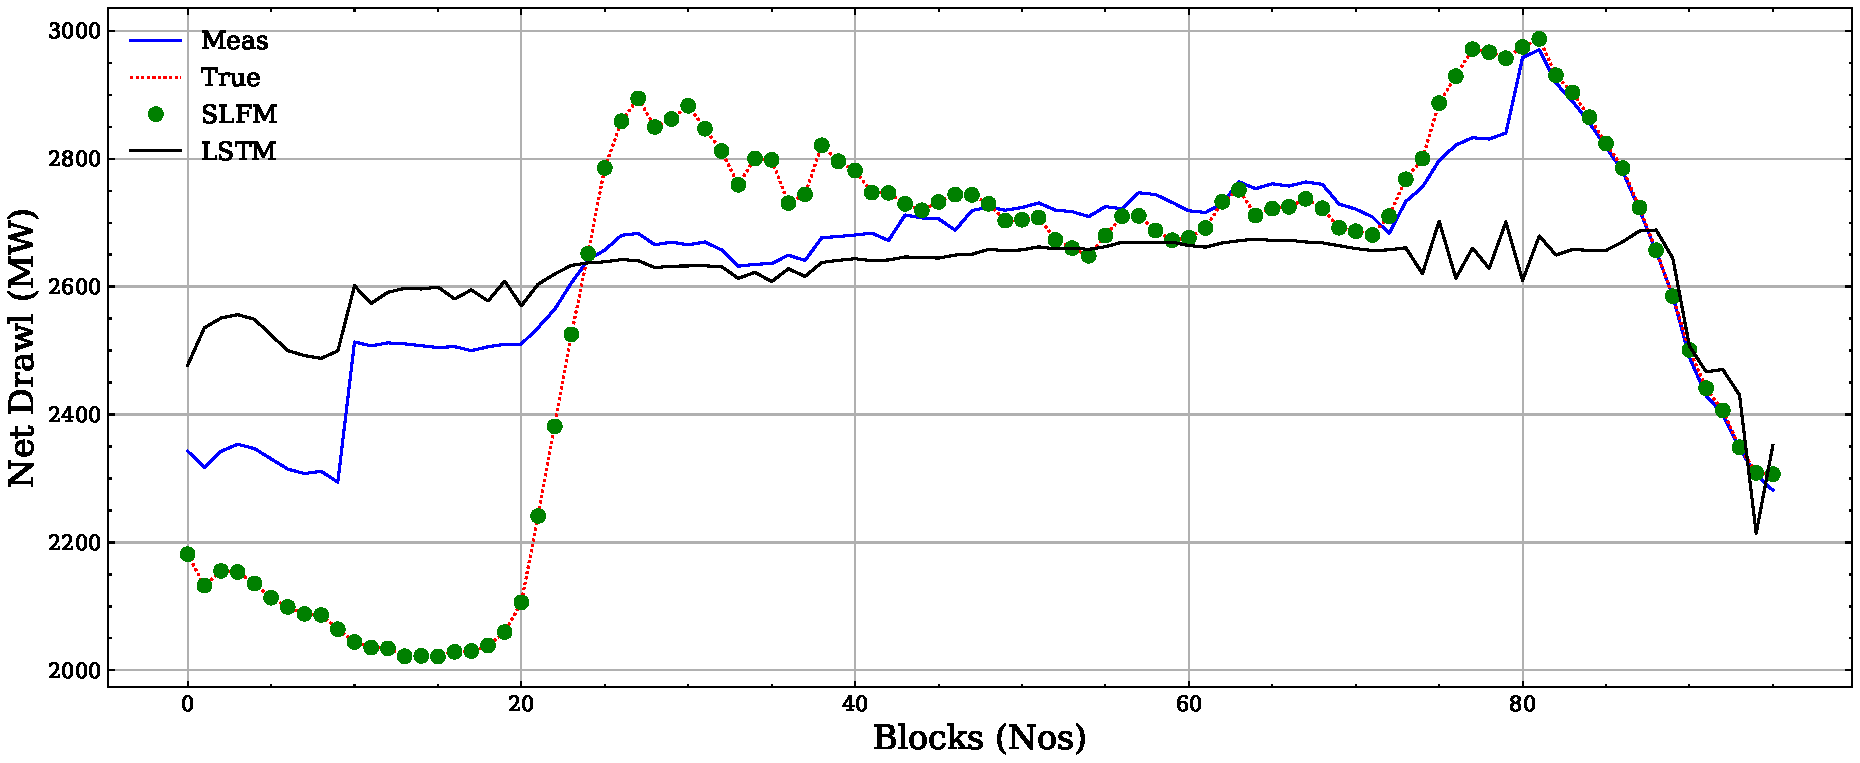
\includegraphics[width=1\linewidth]{Test_results_full1.pdf}
\caption{case-1 comparison of SLFM with LSTM- BAR plot}
\label{case1}
\end{figure}

For case 2, we fed a random (gaussian distribution) data injection to particular parallel feeders, again our method SLFM achieved perfect recall with the minim distance 49, fig \ref{case2}.\\

\begin{figure}[!ht]
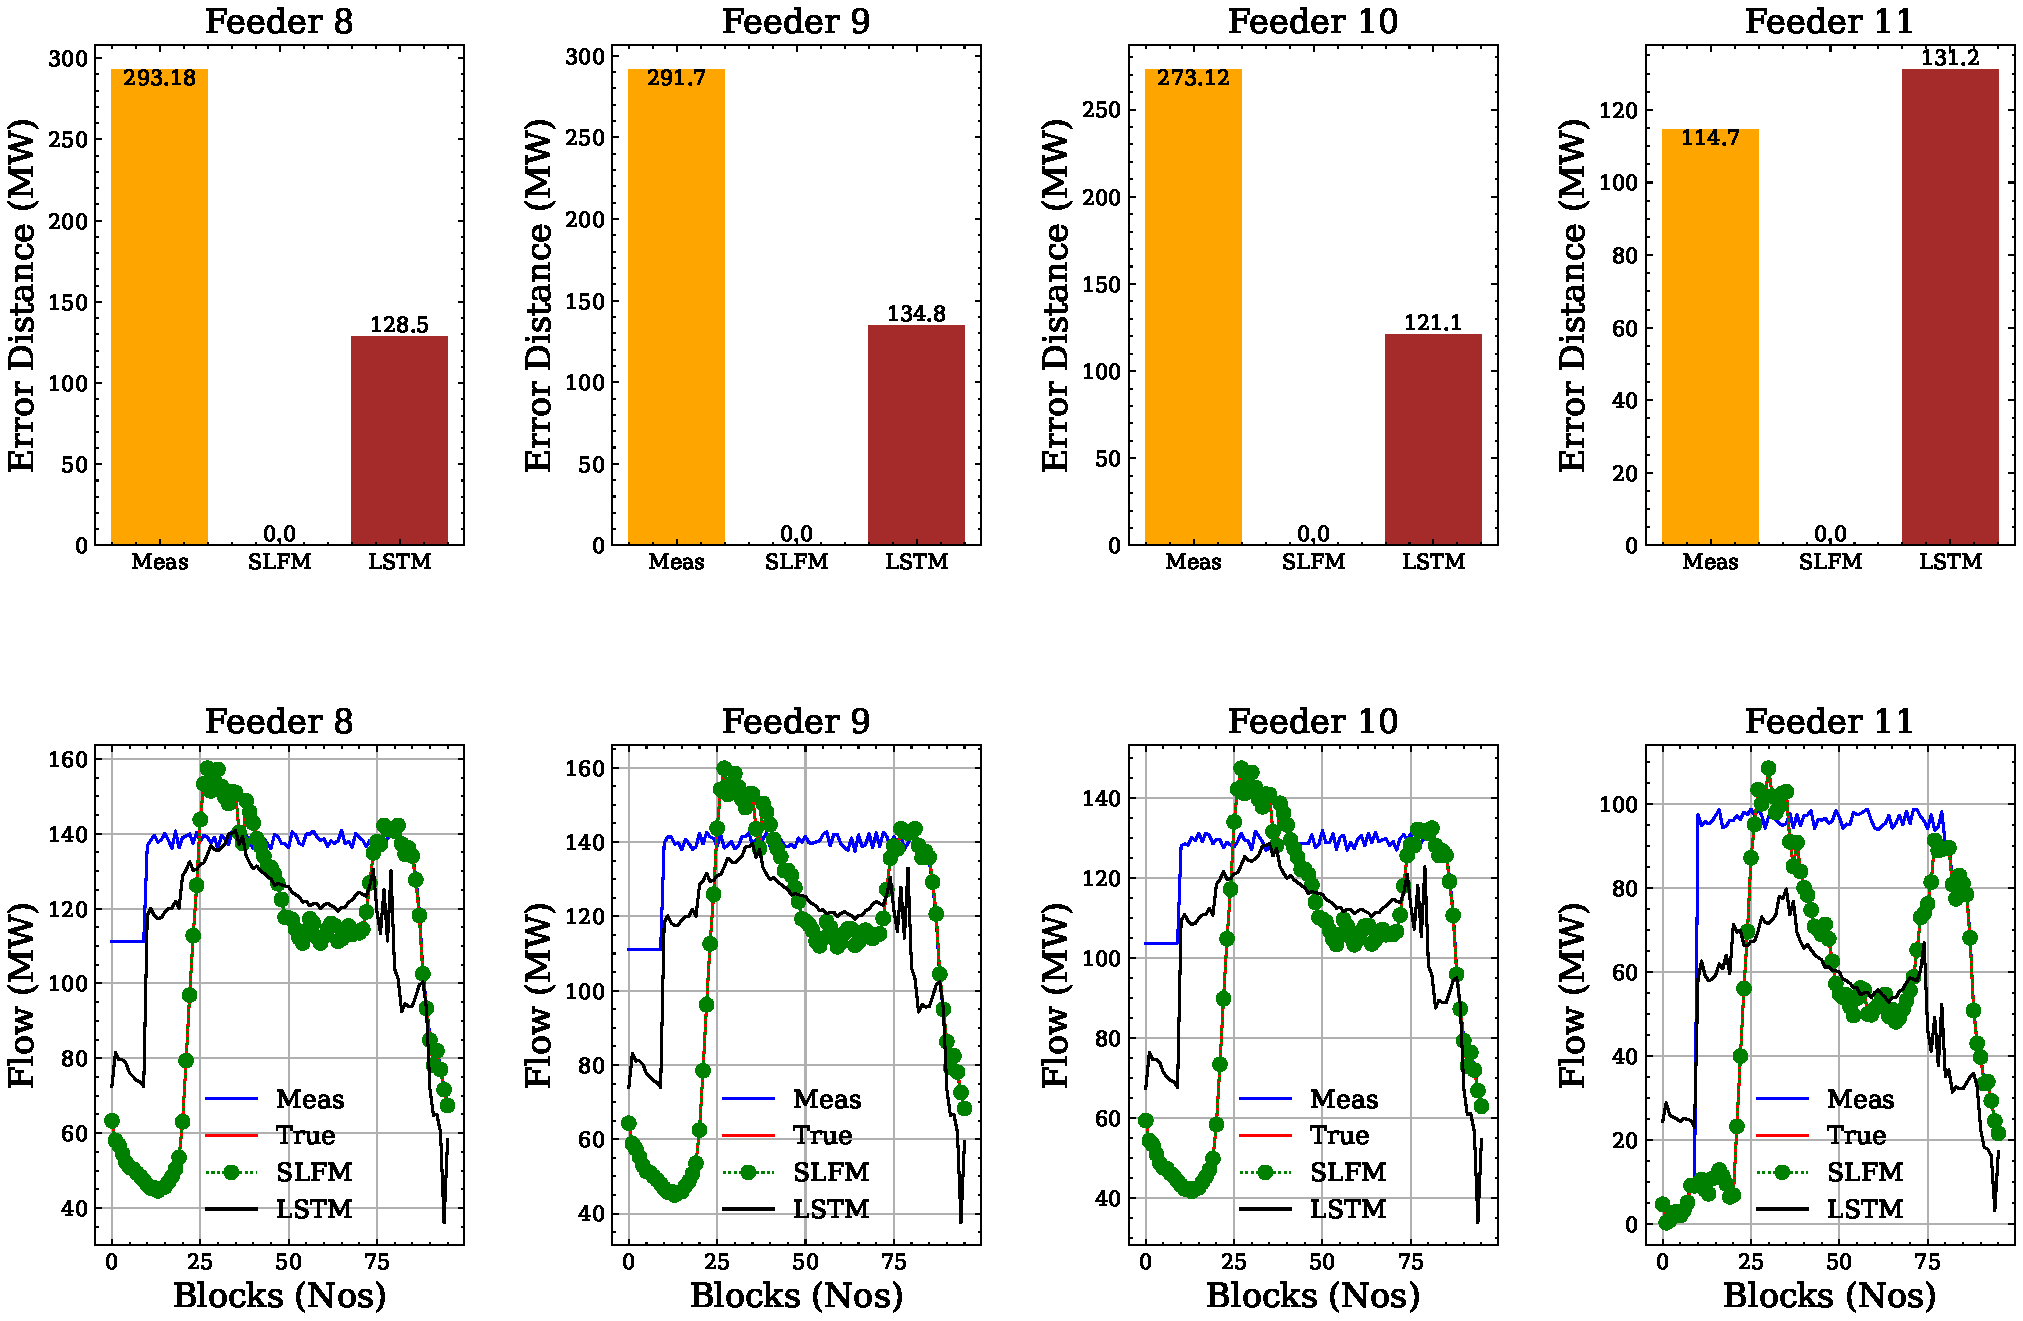
\includegraphics[width=1\linewidth]{Test_results12.pdf}
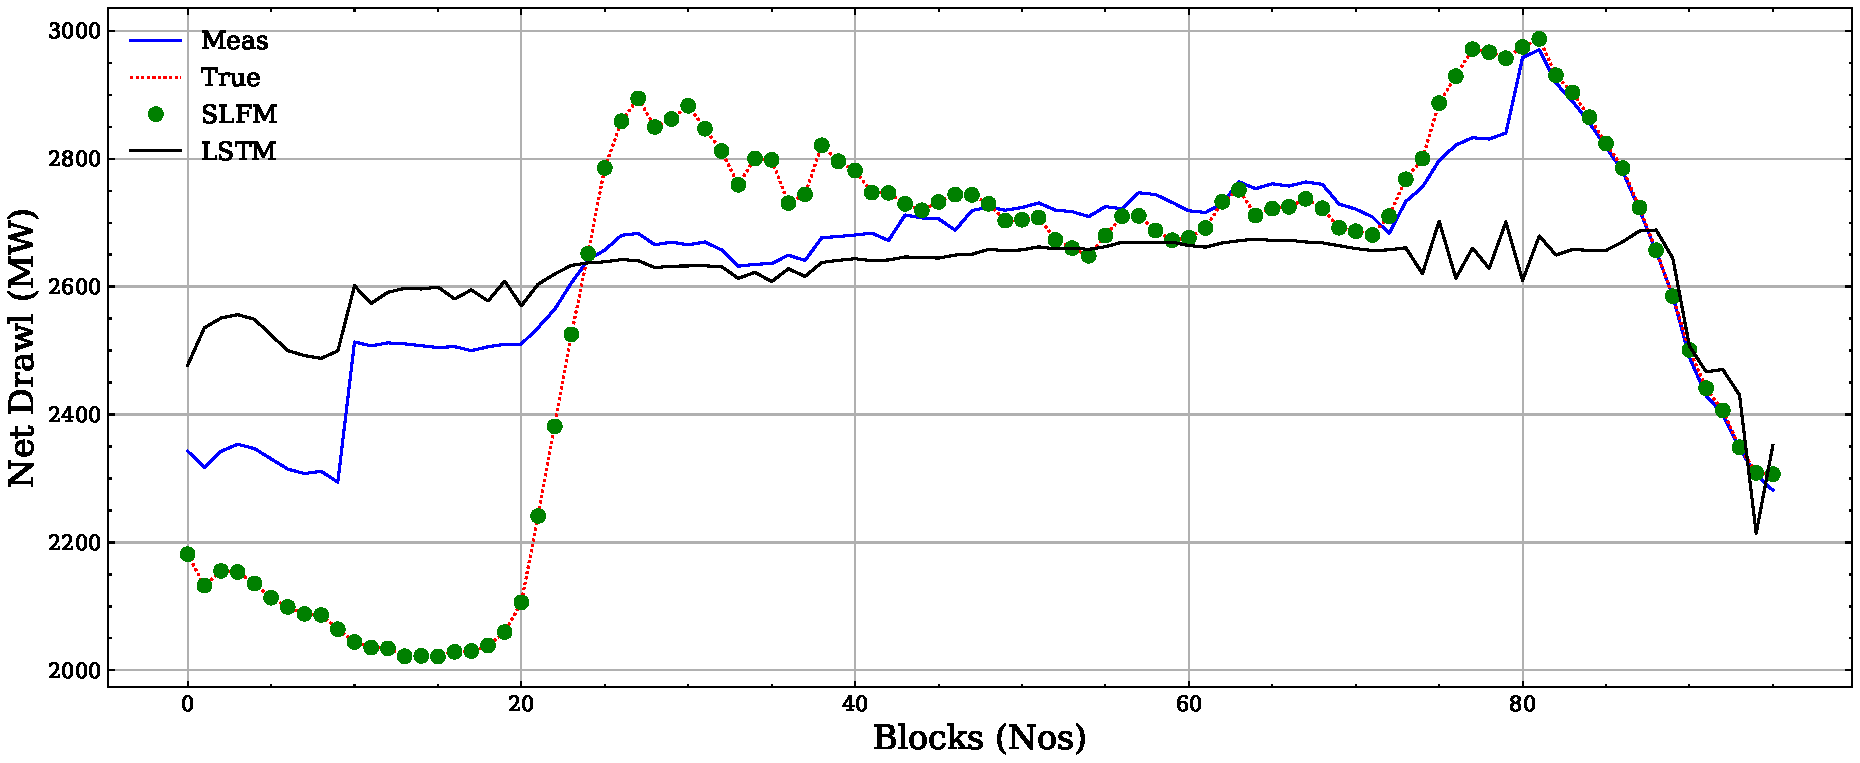
\includegraphics[width=1\linewidth]{Test_results_full2.pdf}
\caption{case-2 comparison of SLFM with LSTM- Line plot}
\label{case2}
\end{figure}

For case 3, unknown disturbance, where that incident signature is not in the stored database, hence the perfect recall is not possible. However, the model (SLFM) achieved better and in line with the standard LSTM Auto-encoder technique , fig \ref{case3}.\\
\begin{figure}[!ht]
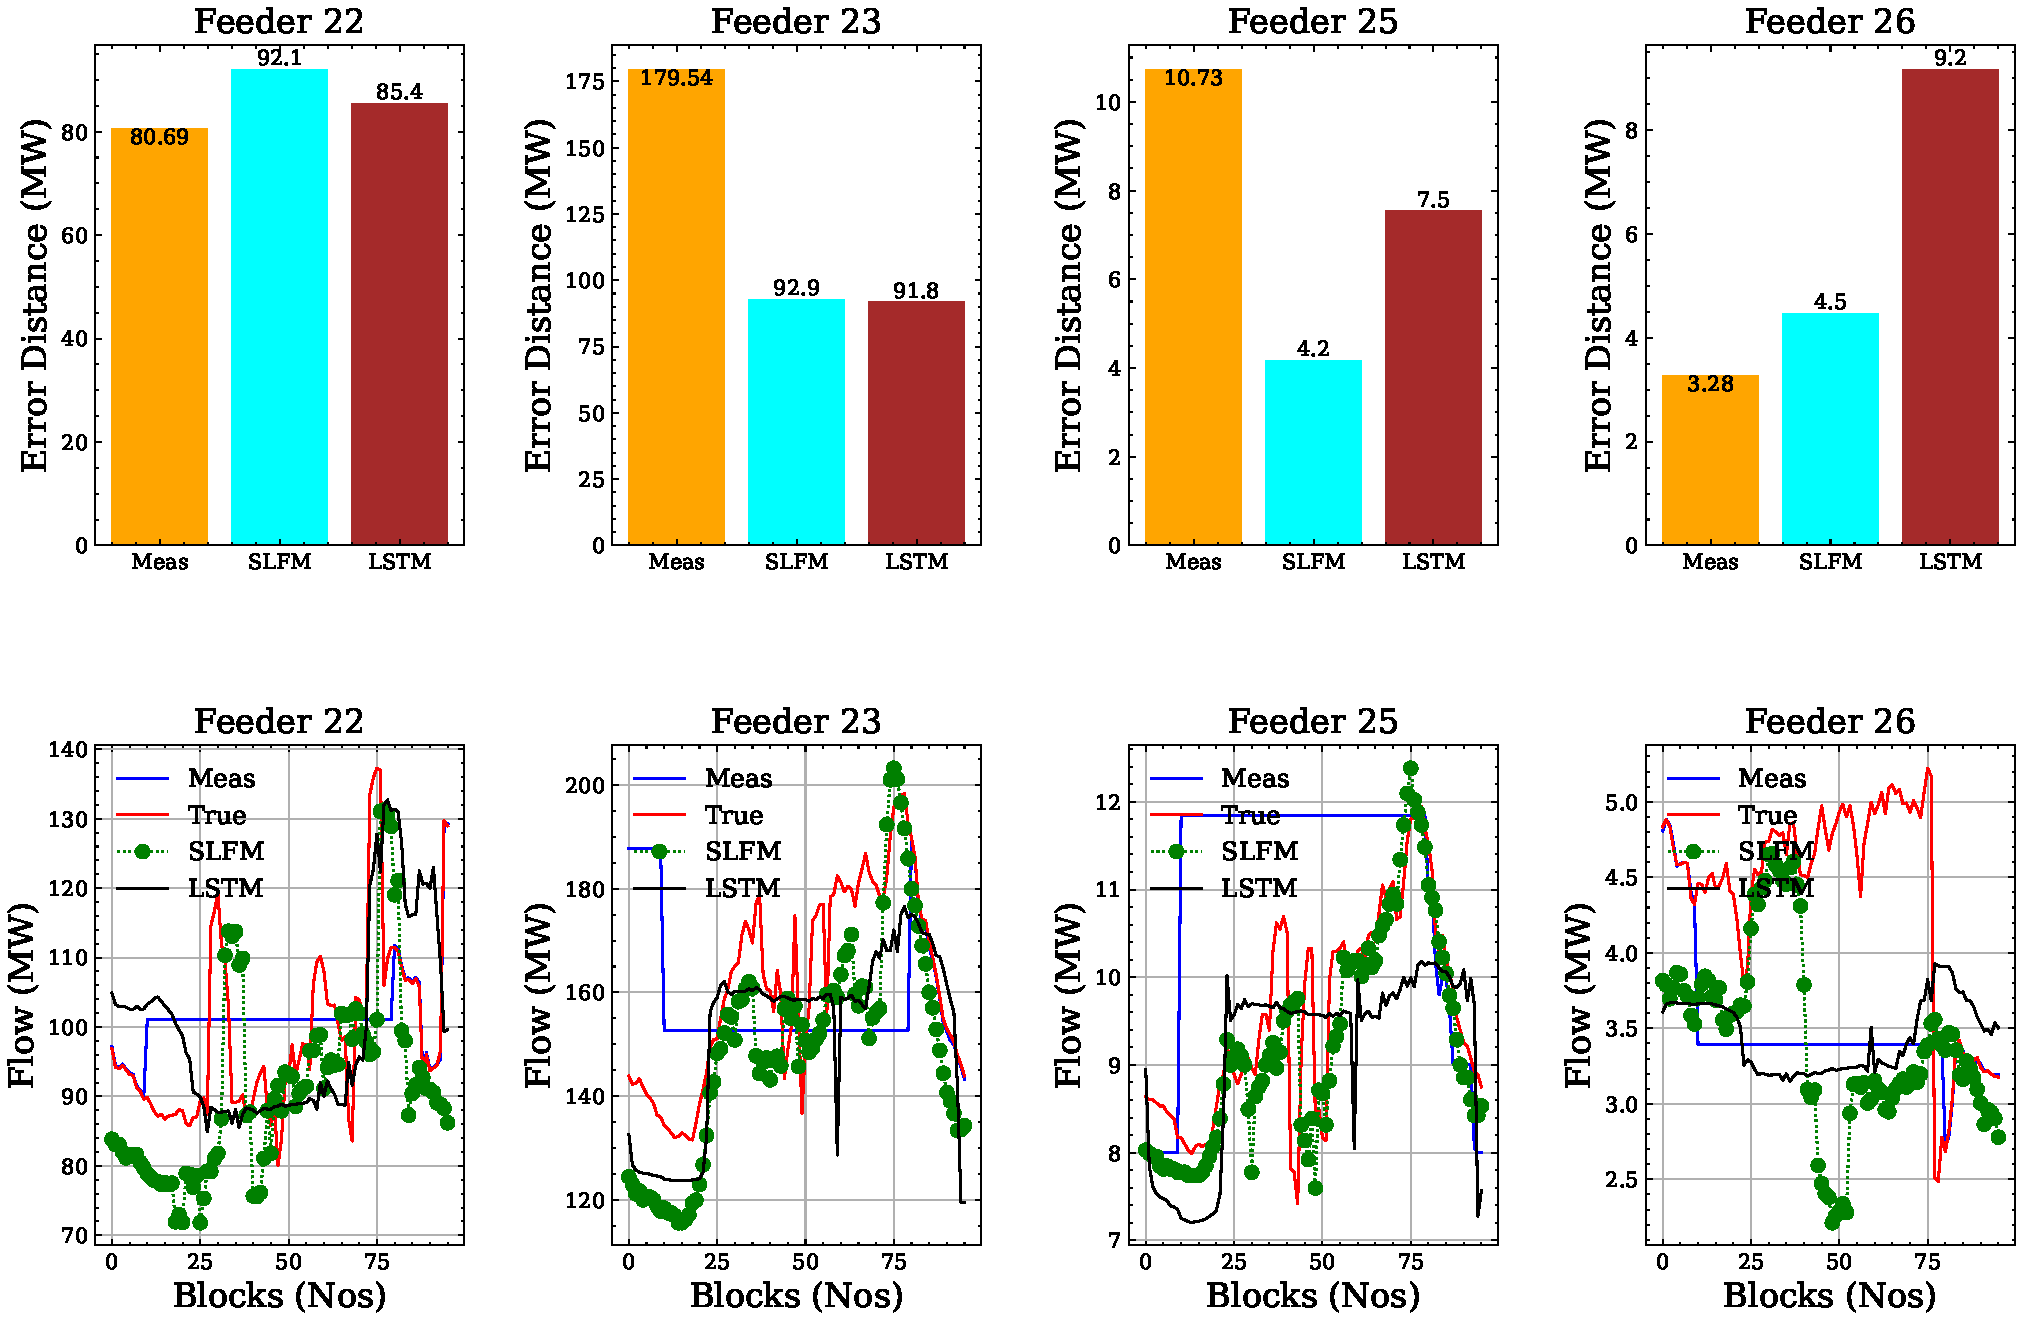
\includegraphics[width=1\linewidth]{Test_results13.pdf}
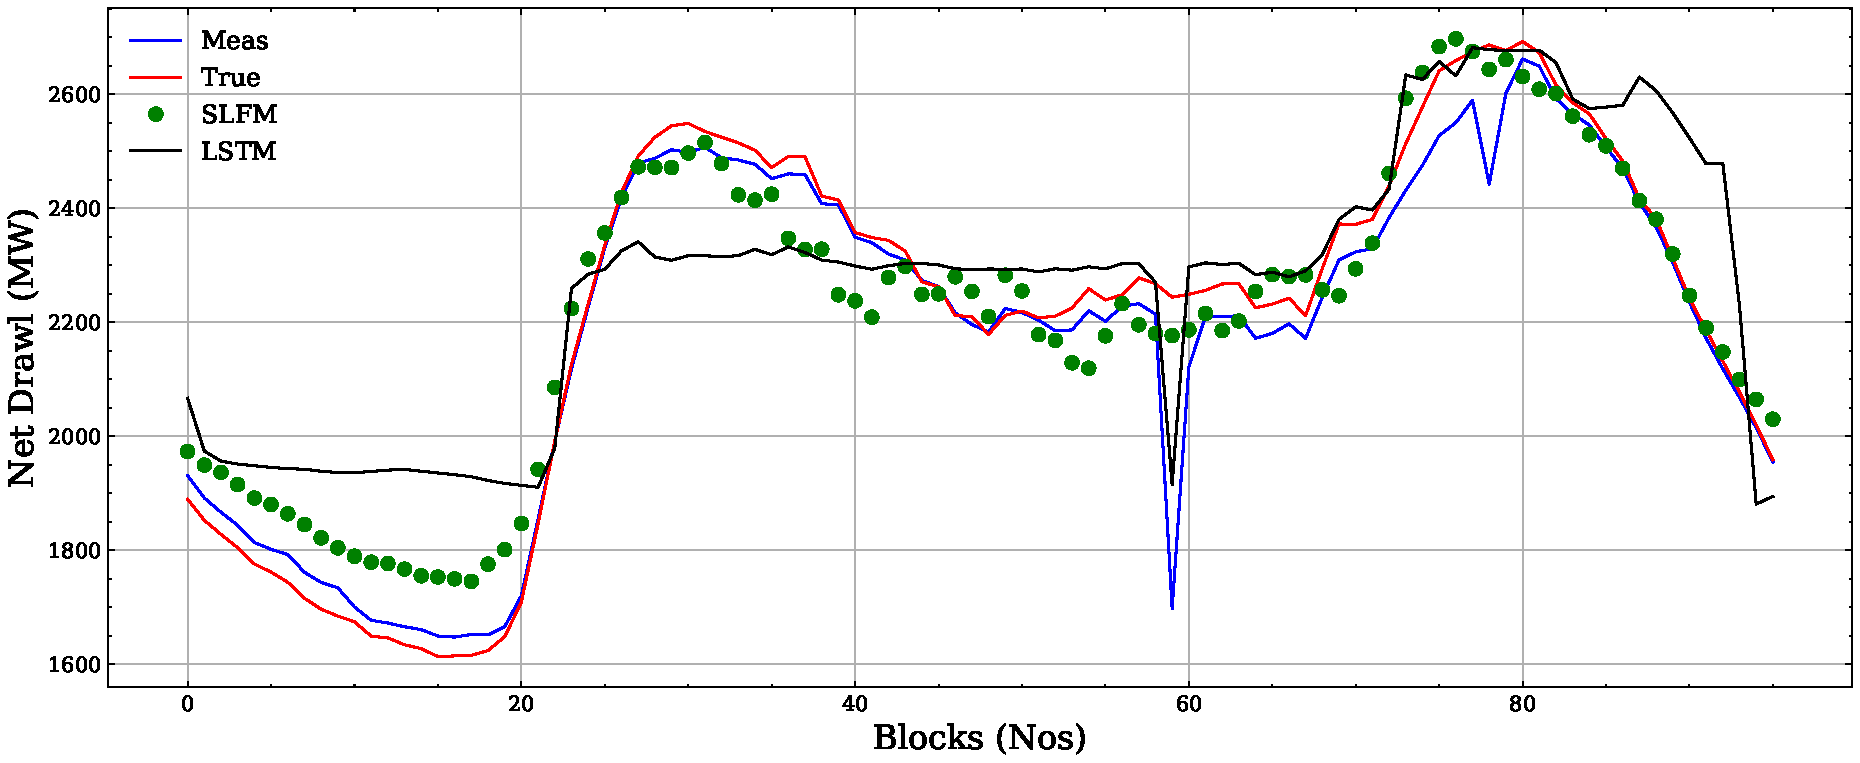
\includegraphics[width=1\linewidth]{Test_results_full3.pdf}
\caption{case-3 comparison of SLFM with LSTM- Line plot}
\label{case3}
\end{figure}

For case 4, Real-time SCADA data collected and fed to the model, and it perfectly captures the true flow and even identifies and estimated the feeder 16 data with minimum error, fig \ref{case4a}-\ref{case4b}.\\

\section{CONCLUSION}
In this paper, we motivated the application of DTW in similarity measurements between time series data and proposed (SLFM) an associative memory technique model for the time series corrupt data estimation problem. We further compared the different case results with the machine learning-based algorithm (LSTM+Autoconder) model. The proposed model defeats the ML models not only in accuracy but also in interpretability, robustness and guarantee in convergence. Further, we are in the process of combining GAN model with SLFM such that the gap between database points be reduced by filling it with generative points.

\begin{figure}[!ht]
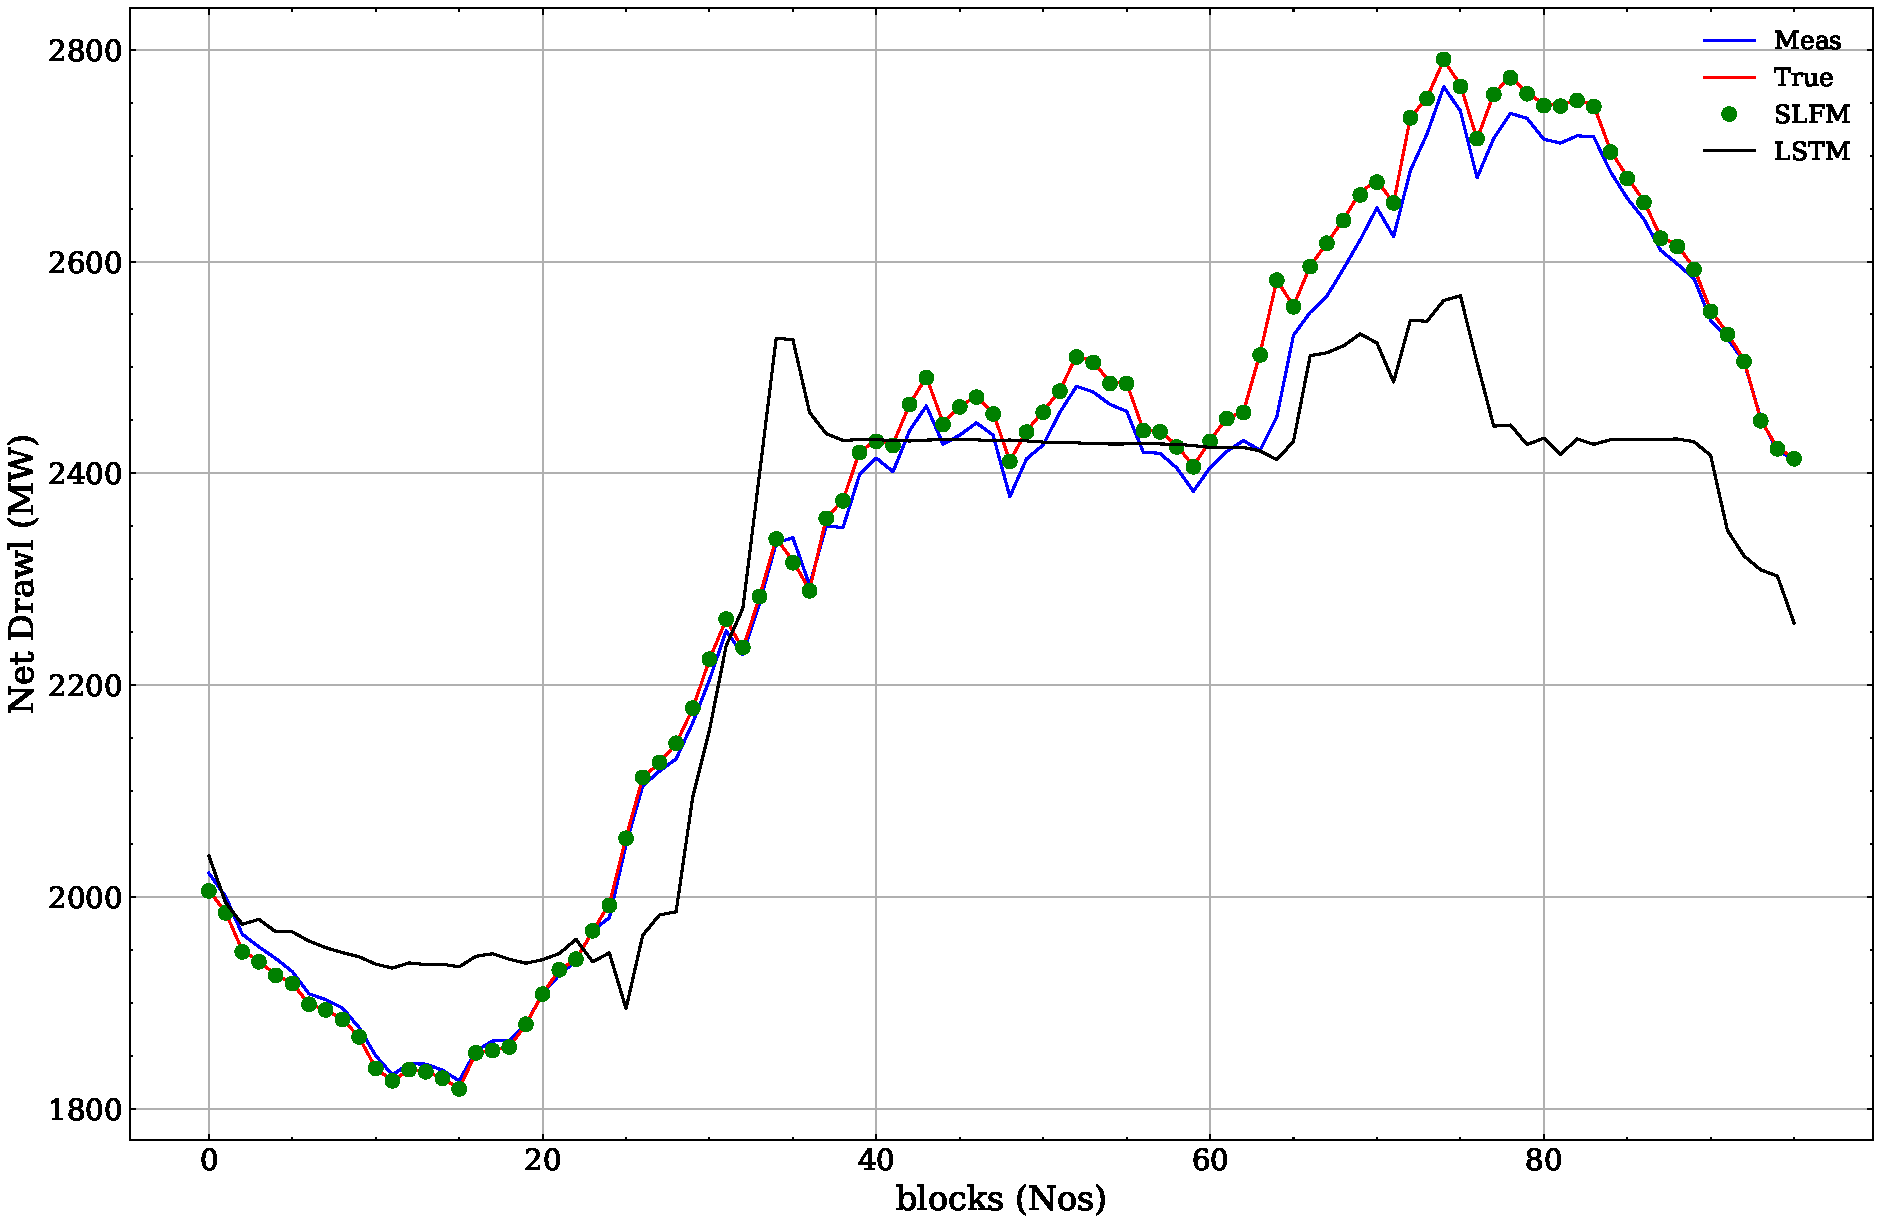
\includegraphics[width=1\linewidth]{Test_results_full5.pdf}
\caption{case-4a comparison of Drawl SLFM with LSTM- Line plot}
\label{case4a}
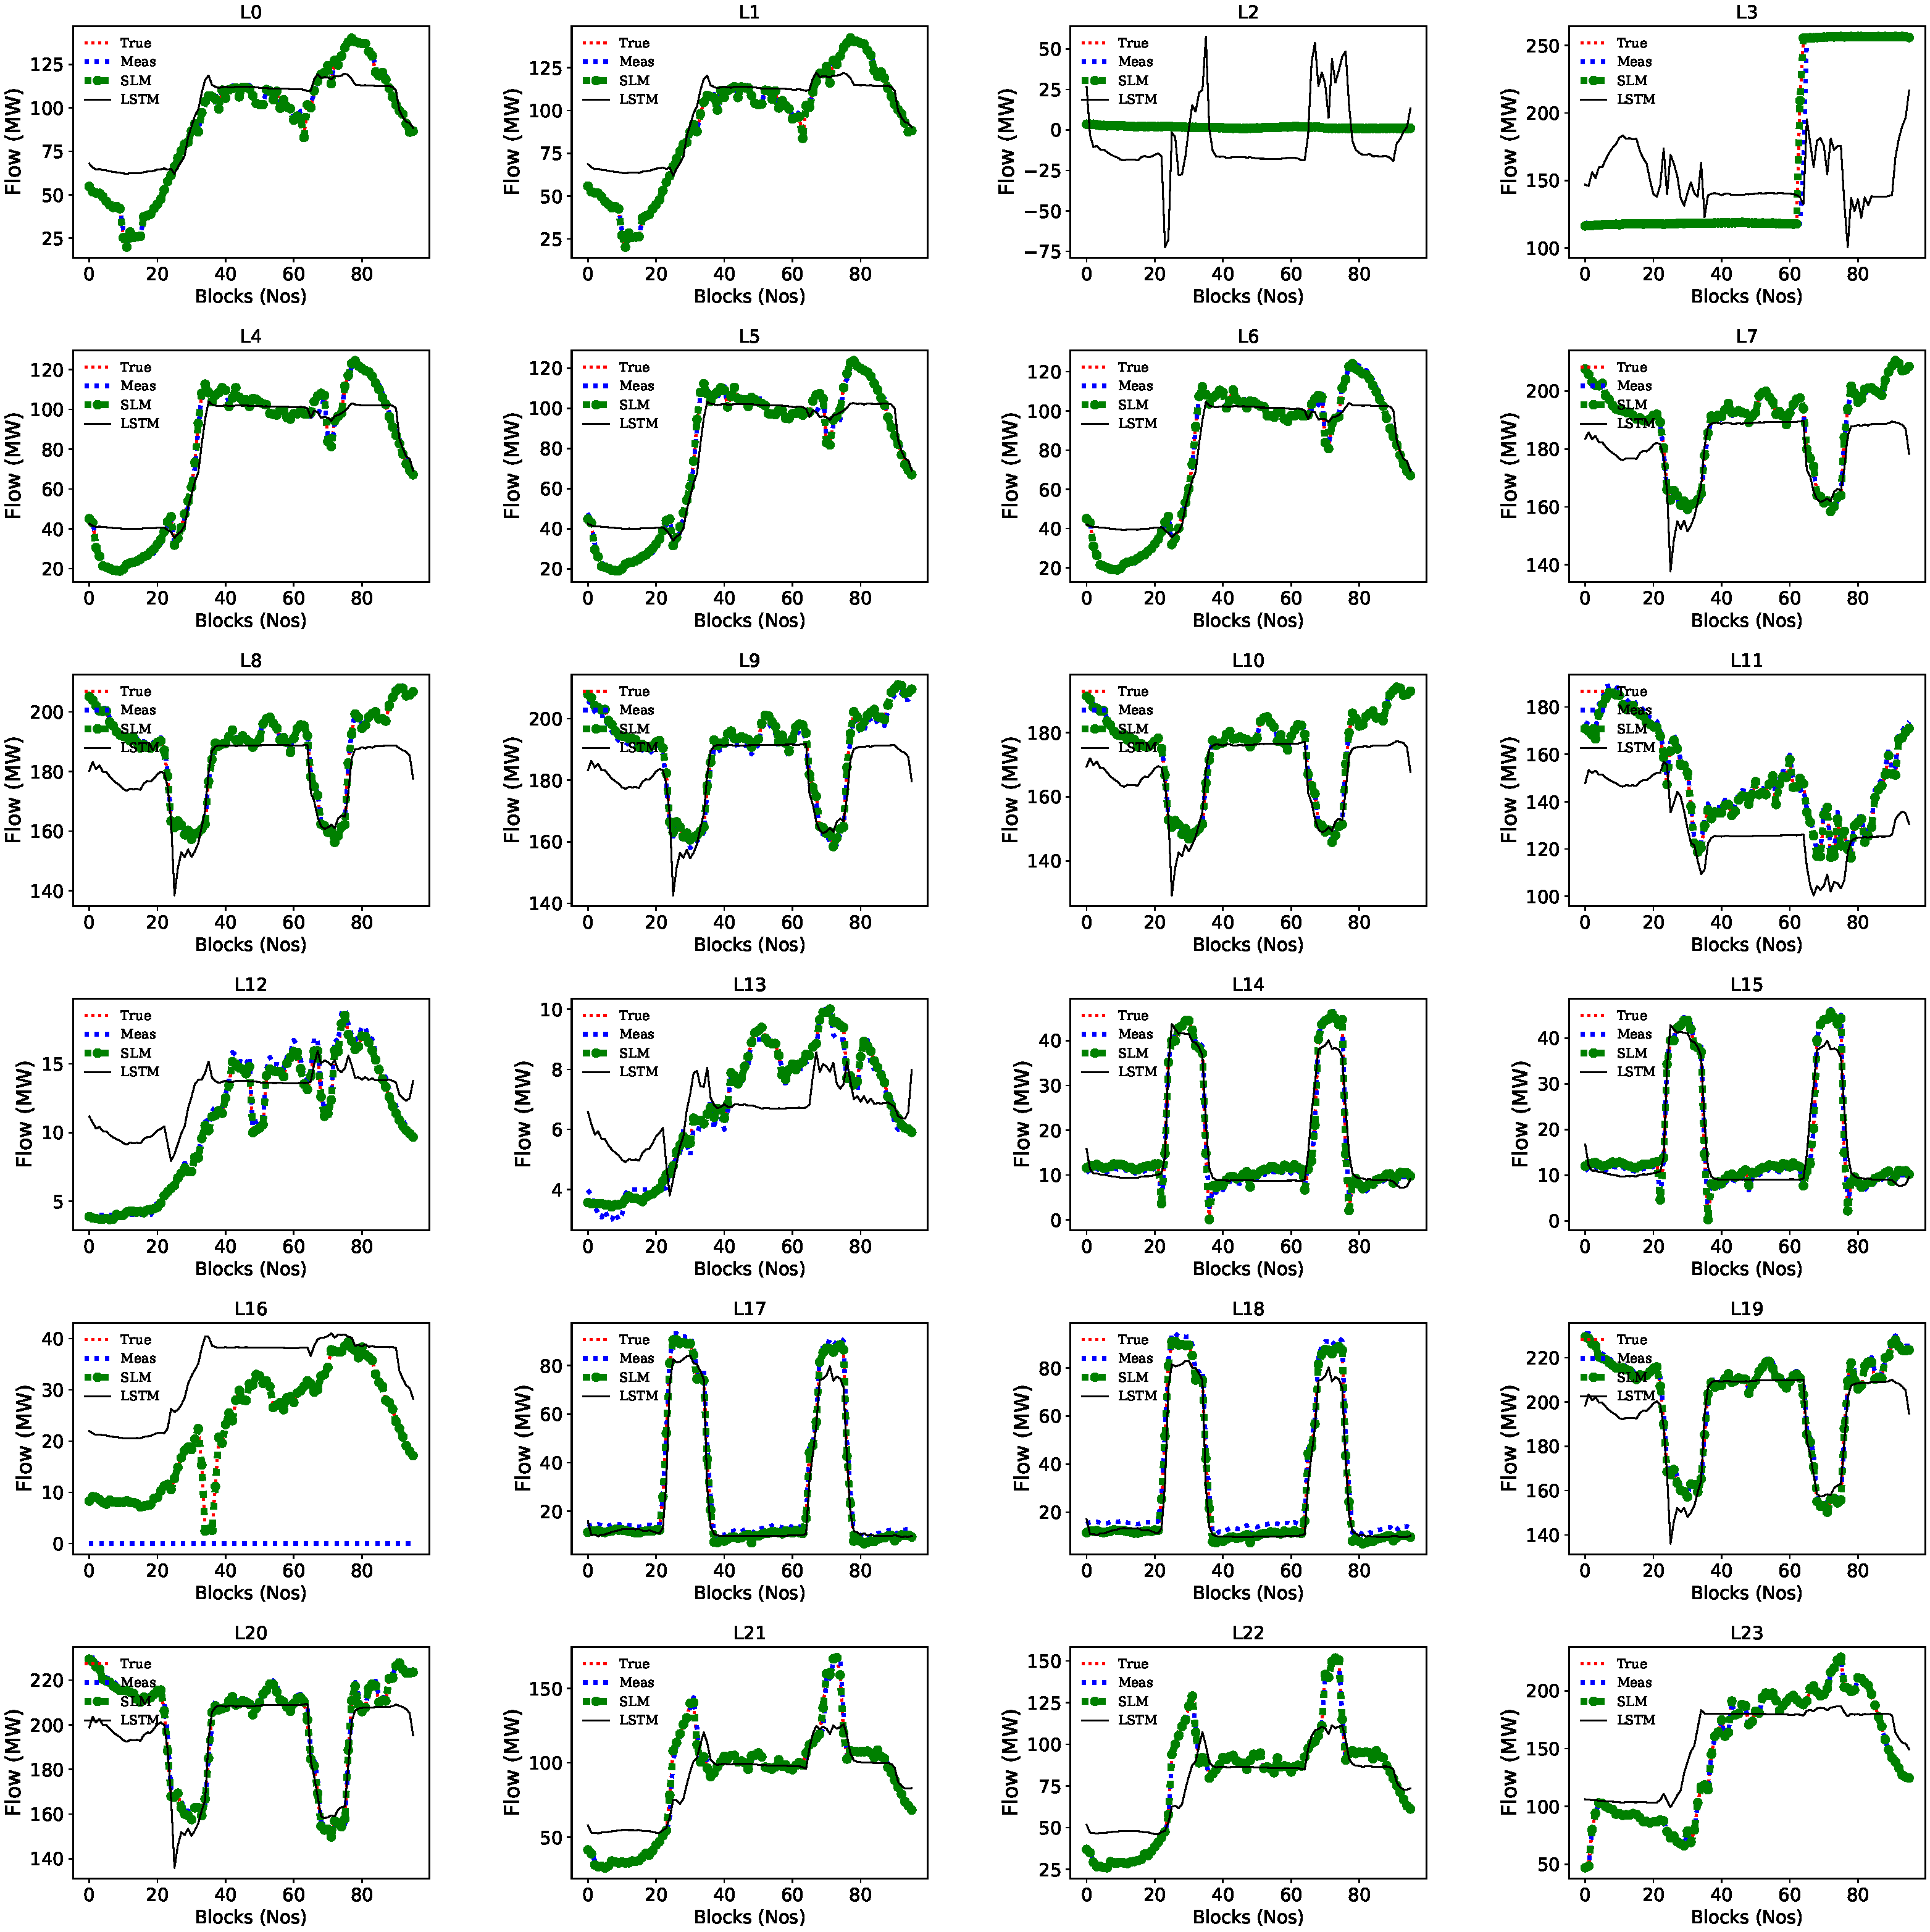
\includegraphics[width=1\linewidth]{Test_results2.pdf}
\caption{case-4b comparison of flow SLFM with LSTM- Line plot}
\label{case4b}
\end{figure}
\begin{comment}
\begin{figure}[!ht]
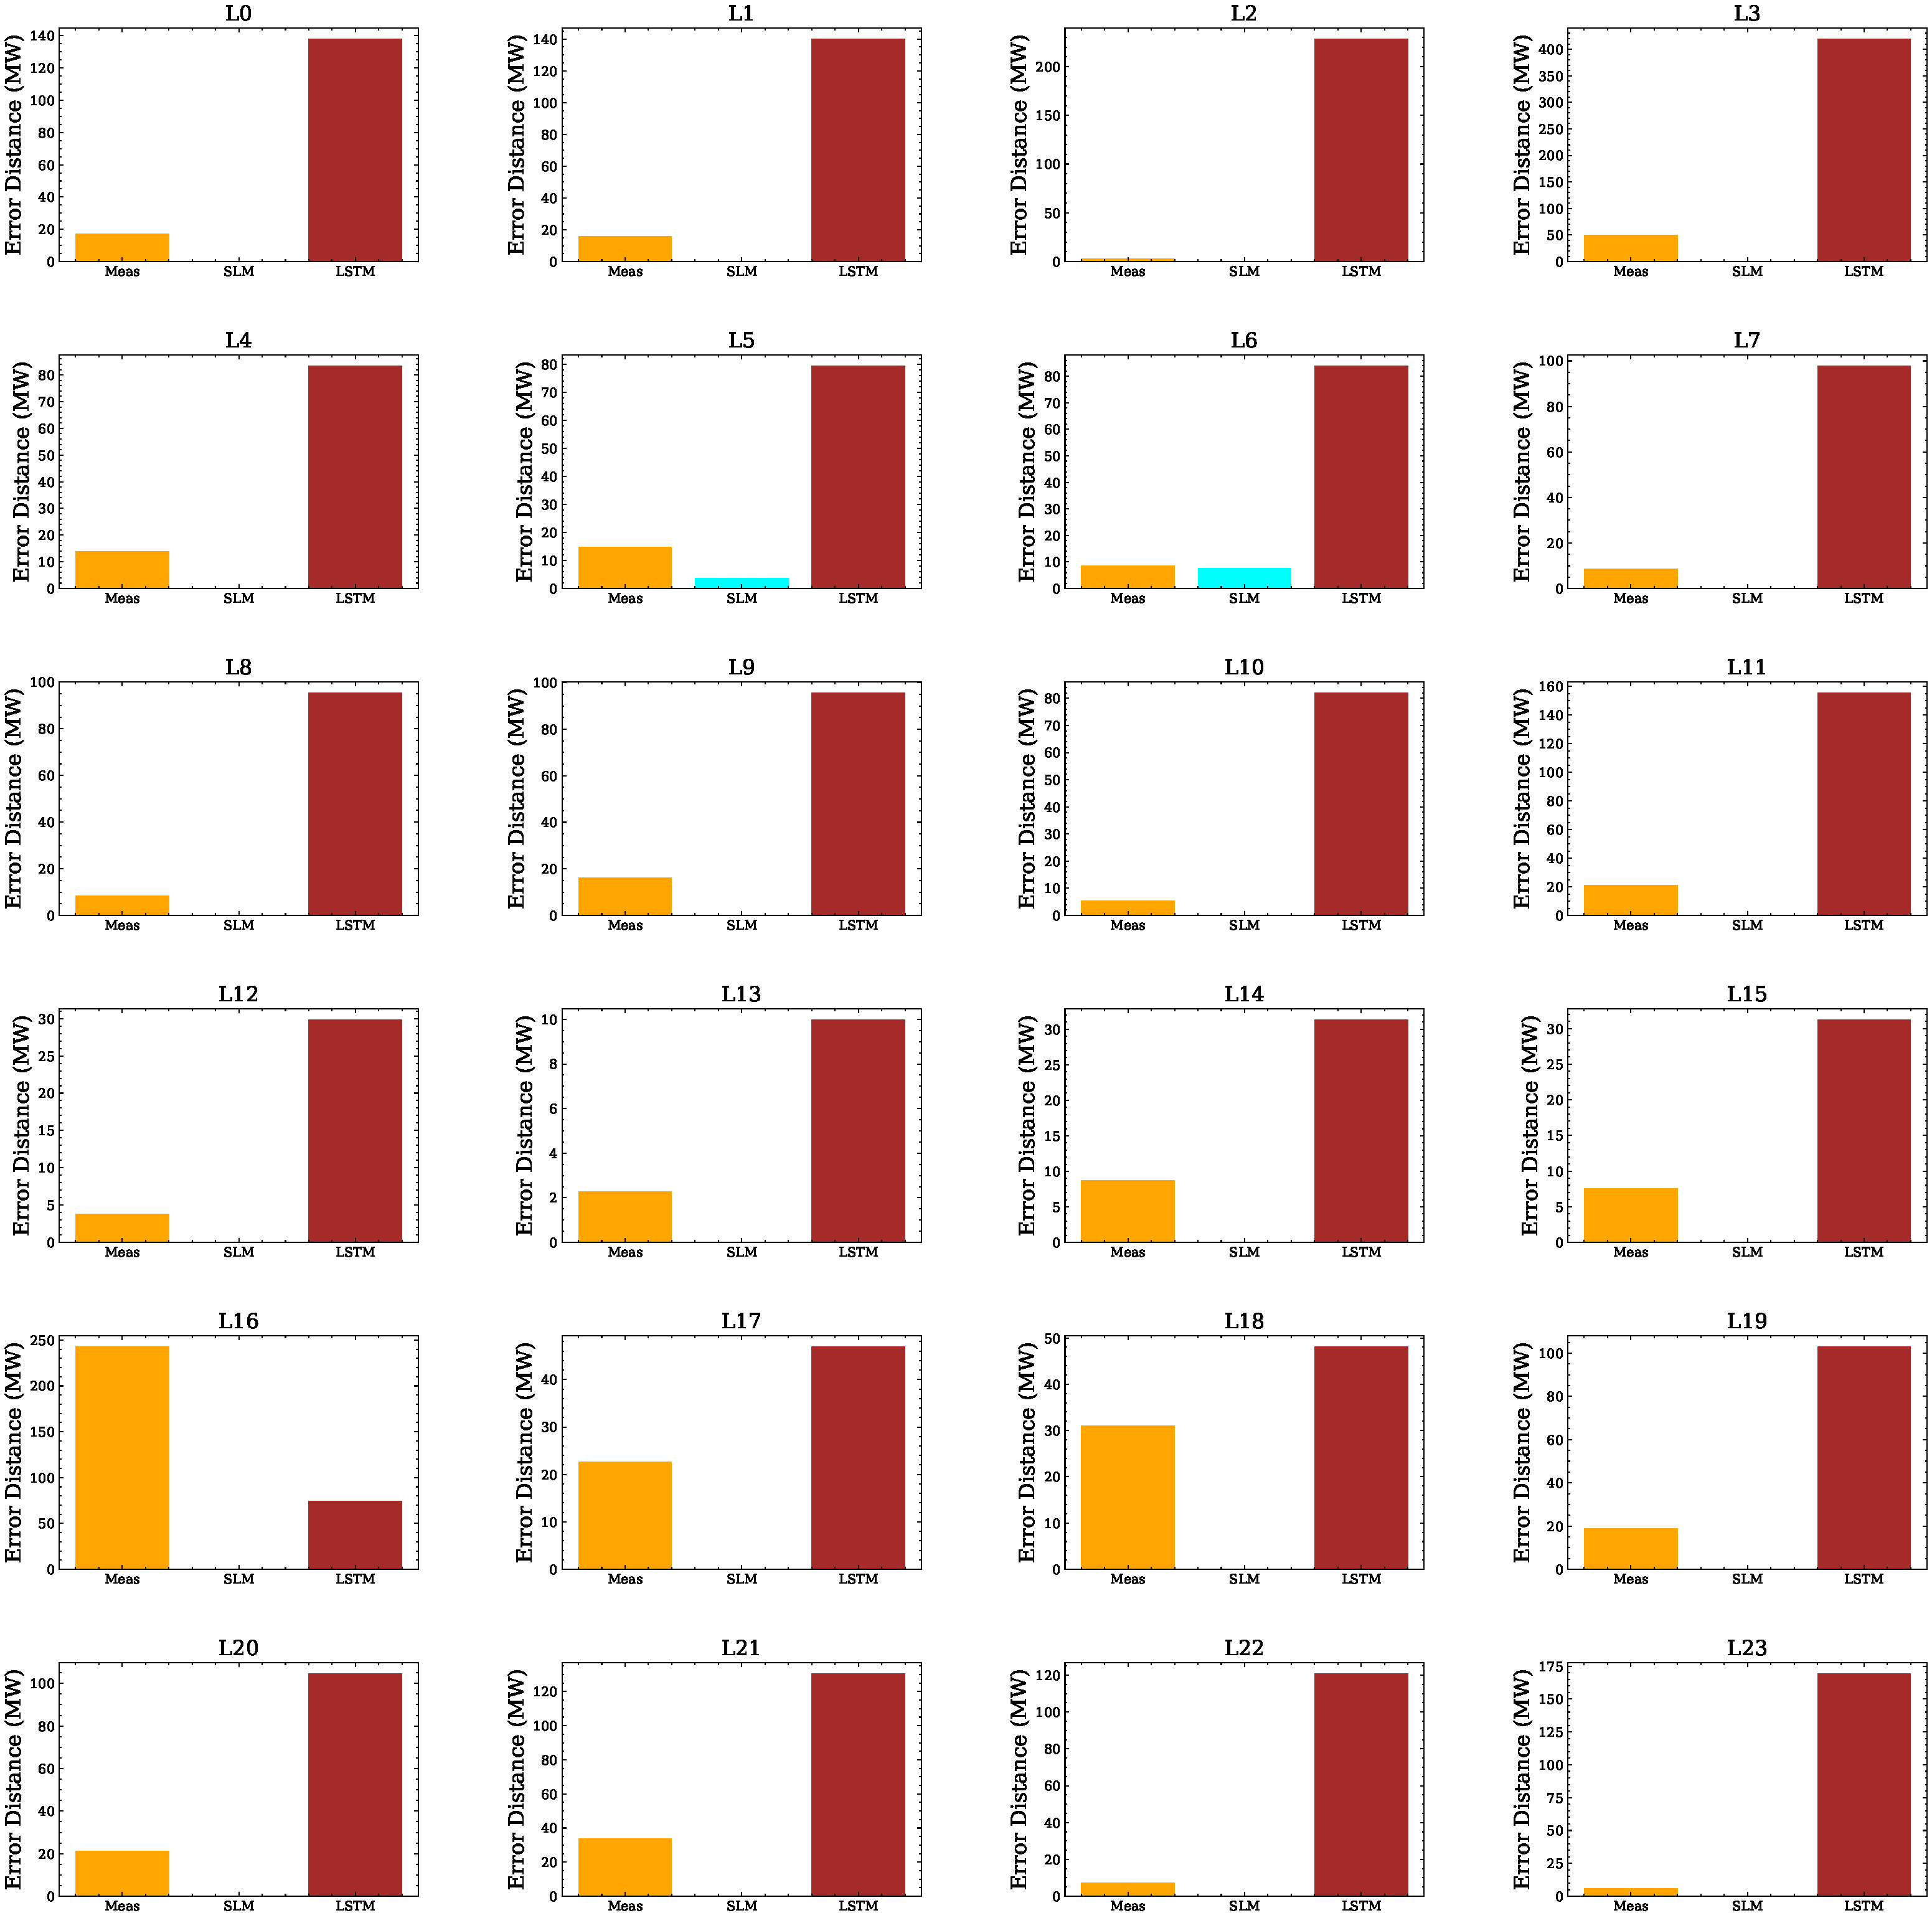
\includegraphics[width=1\linewidth]{Test_results1.pdf}
\caption{case-4c comparison of SLFM with LSTM- BAR plot}
\end{figure}
\begin{figure}[!ht]
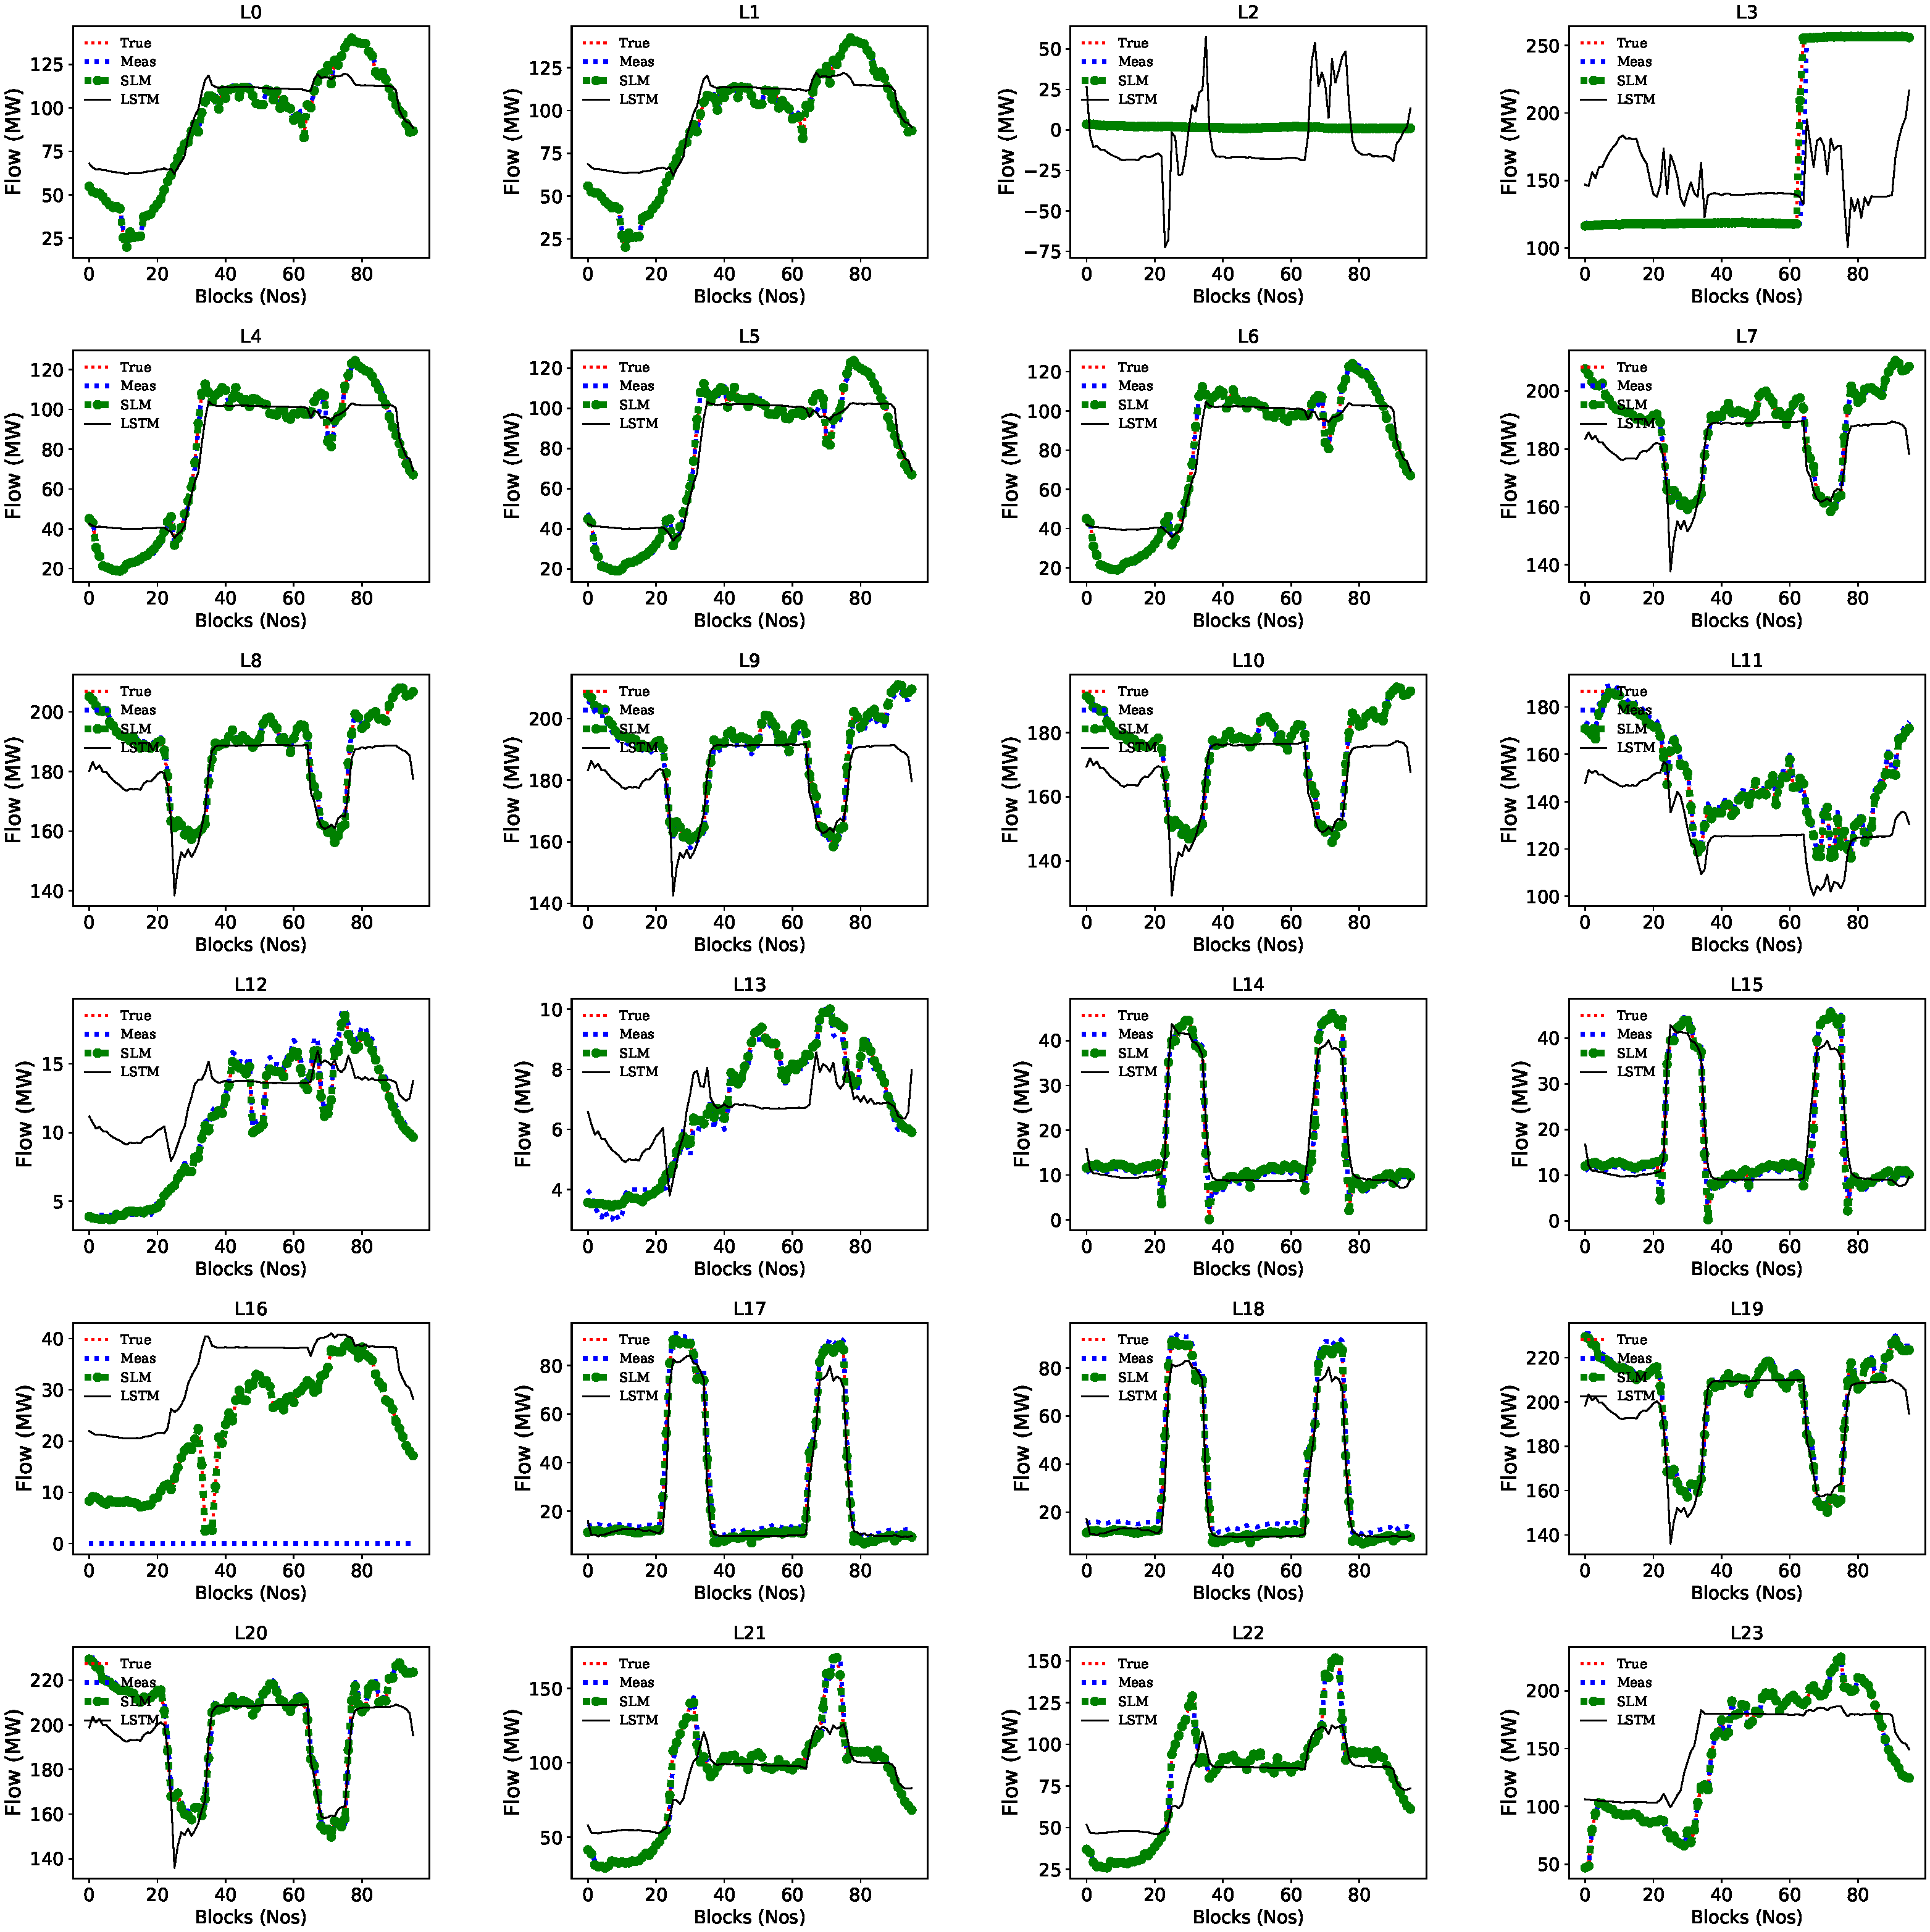
\includegraphics[width=1\linewidth]{Test_results2.pdf}
\caption{case-4b comparison of SLFM with LSTM- Line plot}
\end{figure}
\end{comment}
\section{ACKNOWLEDGMENT}
The authors acknowledge the support and inspiration received from the POSOCO management in publication of this paper. The authors are grateful to their NRLDC colleagues for their liberal contributions for enriching the content in this paper. The views  expressed in this paper are that of the authors and may or may not represent the views of the organization to which they belong. \\ 
%\clearpage
\section*{Appendix-1}
\subsection{proof that associative memory retrieves data- Under well separated }
Consider the space-time series $X$ in $R^{nxd}$ where suspected drawl feeder $x_i \ \in \ X$ and the database of stored patterns be $D_i \in D^{Lxnxd}$ and the $L$ patterns are uncorrelated.
\begin{align*}
& x^{t+1}_j=x^t_j+\frac{\partial x^t_j}{\partial {x^{t-1}}_j}(x^{t-1}_j-x^{t-2}_j) \notag\\
& \frac{\partial x^t_j}{\partial {x^{t-1}_j}}=D^T(diag(P^{t-1})-P^{t-1}(P^{t-1})^T)\frac{\partial S(D_k ,x^{t-1}_j)}{\partial {x^{t-1}_j}} \tag{4} \\
& \text {where } P^{t-1}_i= softmax(S(D_,x^{t-1}_j))= \frac{e^{(S(D_i,{x_j^{t-1}}))}}{\sum_k e^{(S(D_k ,{x_j^{t-1}}))}} \\
&=\frac{1}{1+\sum_{k!=j} e^{(S(D_k ,{x_j^{t-1}})-S(D_i ,{x_j^{t-1}}))}} \\
&=\frac{1}{1+\sum_{k!=j}e^{-\delta_k}} \sim \frac{1}{1+({N-1)}*e^{-\delta_c} } \sim 1\\
&\because \text{datapoints are well separated } \text{max} \delta_k =\delta_c>>0 \\ 
& \text{ i.e  the corupted point has higher similar and} \\
& \text{lower distance to the database point i.} \\
&P^{t-1}_r=softmax(S(D_r,x^{t-1}_j)) =\frac{e^{(S(D_r,{x_j^{t-1}}))}}{\sum_k e^{(S(D_k ,{x_j^{t-1}}))}} \\
&=\frac{e^{(S(D_r ,{x_j^{t-1}})-S(D_i ,{x_j^{t-1}}))}}{1+\sum_{k!=j} e^{(S(D_k ,{x_j^{t-1}})-S(D_i ,{x_j^{t-1}}))}} \\
& = \frac{e^{-\delta_c}}{1+({N-1)}*e^{-\delta_c} }\\
& \sim 0 \because e^{\delta_c} \ge 0 \\
&\text{now } P^{t-1}=[P^{t-1}_r , P^{t-1}_i]=[0, 1] \\
\end{align*}

$diag(P^{t-1})-(P^{t-1})^TP^{t-1}$=\[
\begin{bmatrix}
 0     & 0 \\
  0        &  1 \\
\end{bmatrix}
-
\begin{bmatrix}
 0      & 0 \\
  0     &  1 \\
\end{bmatrix}
=
\begin{bmatrix}
 0      & 0 \\
  0       &  0 \\
\end{bmatrix}
\]
\begin{align*}
& \frac{\partial x^t_j}{\partial {x^{t-1}}_j}= diag(P^{t-1})-P^{t-1}(P^{t-1})^T= constant\\
& \frac{\partial x^{t+1}_j}{\partial {x^{t}}_j}=0 \\
& \text{ point converged to unique point, after second iteration} 
\end{align*}

\begin{thebibliography}{00}
\bibitem{b7} J. F. Rendon-Sanchez and L. M. de Menezes, "Structural combination of seasonal exponential smoothing forecasts applied to load forecasting", Eur. J. Oper. Res., vol. 275, no. 3, pp. 916-924, Jun. 2019.
\bibitem{b8} F. Bashir and H. Wei, "Neurocomputing Handling missing data in multivariate time series using a vector autoregressive model-imputation ( VAR-IM ) algorithm", Neurocomputing, vol. 276, pp. 23-30, 2018
\bibitem{b16} I. Markovsky. "Algorithms and literate programs for weighted low-rank approximation with missing data", volume 3 of Springer Proc. Mathematics, pages 255–273. Springer, 2011
\bibitem{b6} S. Ryu, M. Kim and H. Kim, "Denoising autoencoder-based missing value imputation for smart meters", IEEE Access, vol. 8, pp. 40656-40666, 2020.
\bibitem{b1}  L. Liu, M. Esmalifalak, Q. Ding, V. A. Emesih, and Z. Han, “Detecting false data injection attacks on power grid by sparse optimization,” IEEETransactions on Smart Grid, vol. 5, no. 2, pp. 612–621, 2014.
\bibitem{b2} Y. He, G. J. Mendis, and J. Wei, “Real-time detection of false data injection attacks in smart grid: A deep learning-based intelligent mechanism,” IEEE Transactions on Smart Grid, vol. 8, no. 5, 2017.
\bibitem{b3} Jinsung Yoon, William R. Zame, Mihaela van der Schaar, "Estimating Missing Data in Temporal Data Streams Using Multi-Directional Recurrent Neural Networks," IEEE Transactions on Biomedical Engineering, 2019.
\bibitem{b4} K. Park et al "Missing-Insensitive Short-Term Load Forecasting Leveraging Autoencoder and LSTM", IEEE Acess 10.1109/ACCESS.2020.3036885, Nov 2020
\bibitem{b5} S. A. Foroutan and F. R. Salmasi, “Detection of false data injection attacks against state estimation in smart grids based on a mixture gaussian distribution learning method,” IET Cyber-Physical Systems: Theory \& Applications, vol. 2, no. 4, pp. 161–171, 2017.
\bibitem{b9}  N. Laptev, J. Yosinski, E. Li, and S. Smyl, “Time-series extreme event forecasting with neural networks at uber,” International Conference on Machine Learning, 2017.
\bibitem{b11}Michael Widrich, "Modern Hopfield Networks and Attention for Immune Repertoire Classification", 34th Conference on Neural Information Processing Systems (NeurIPS 2020)
\bibitem{b12}  Hubert Ramsauer, “Hopfield Networks is All You Need,” International Conference on Machine Learning, 2021.
\bibitem{b17} Donald J Berndt and James Clifford. Using dynamic time warping to find patterns in time series.In KDD workshop, volume 10, pages 359–370. Seattle, WA, 1994
\bibitem{b18} Xingyu Cai, "DTWNet: a Dynamic Time Warping Network",Advances in Neural Information Processing Systems, 2020
\bibitem {b10} Romain Tavenard ,"Tslearn, A Machine Learning Toolkit for Time Series Data",Journal of Machine Learning Research 2020,
\bibitem {b13}A. H. Yaacob, I. K. Tan, S. F. Chien, and H. K. Tan, “Arima basednetwork anomaly detection,” in 2010 Second International Conference on Communication Software and Networks. IEEE, 2010, pp. 205–209,
\bibitem{b14} S.N.Ram, "inference Based Latent Space Method for False data and Topology estimation under suspect EMS data", International Conference on Power Electronics and Energy (ICPEE) 2021.
\bibitem{b15}  A. Ashok, M. Govindarasu, and J. Wang, “Cyber-physical attackresilient wide-area monitoring, protection, and control for the power
grid,” Proceedings of the IEEE, vol. 105, no. 7, pp. 1389–1407, 2017.
%\bibitem{b17}CEA, " https://cea.nic.in/wp-content/uploads/regulatory_affairs/2021/02/List_of_deemed_licensees.pdf", dpdf
%\bibitem{b18} \href{ https://www.aperforum.org/files/2020-01-india.pdf}
\end{thebibliography}
\begin{comment}
\section{Bi directional LSTM works}

For the case, we use simple dot product as similarity function  ,i.e $\bf{ D.\psi_{C}}$.

\section{BILSTM with Aoociative memory}

\subsection{BILSTM}[H]
Bi LSTM is sequence processing model that has both Forward and Backward direction of information. Bi derectional helps to find out the dependecies of last word to fist word (in language translation ). Bi LSTM helps to capture  the diference in ramp rates between morning and evening peaks by processing it bi directinally.


is a variant of Recurrent Neural Network (RNN). It can effectively overcome the problem of gradient disappearance in RNN, especially in long-distance tasks, it is significantly better than RNN, and the gradient will not disappear in the process of back propagation. RNN is a chain network with a repeating neural network module. In a standard RNN, this repeated module has only a very simple structure. However, LSTM has the same structure but a gating mechanism is introduced in the repeating module to control the memory and forgetting of information. The network structure diagram is shown as follows \\


\begin{align}
\mathbf{I}_t  &= \sigma(\mathbf{X}_t \mathbf{W}_{xi} + \mathbf{H}_{t-1} \mathbf{W}_{hi} + \mathbf{b}_i),\\
\mathbf{F}_t  &= \sigma(\mathbf{X}_t \mathbf{W}_{xf} + \mathbf{H}_{t-1} \mathbf{W}_{hf} + \mathbf{b}_f), \\
\tilde{\mathbf{C}}_t &= \text{tanh}(\mathbf{X}_t \mathbf{W}_{xc} + \mathbf{H}_{t-1} \mathbf{W}_{hc} + \mathbf{b}_c),\\
\mathbf{O}_t  &= \sigma(\mathbf{X}_t \mathbf{W}_{xo} + \mathbf{H}_{t-1} \mathbf{W}_{ho} + \mathbf{b}_o) \\
\mathbf{C}_t &= \mathbf{F}_t \odot \mathbf{C}_{t-1} + \mathbf{I}_t \odot \tilde{\mathbf{C}}_t.\\
\mathbf{H}_t & = \mathbf{O}_t \odot \tanh(\mathbf{C}_t).
\end{align}
\end{comment}
%then $\exists$ $T^{kxd}$ (estimated  measurement) be perfect  when $T \subset M \subset D_M$  %
\begin{comment}
\begin{align*} 
\phi^*,\psi^* =\underset{\phi,\psi}{\text{min}} \  ||\sum_k\psi(\phi(z^{sc}_k,D_S),D_M)- z^m_k|| \ \because  z^{sc}_{j:k,T} \in C \\
 z^{*{sc}}_{j:k,T} = \psi^*(\phi^{*}(z^{sc}_k,D_S),D_M) \because  z^{*{sc}}_{j:k,T} \in T \\
\end{align*}

\subsection{Dynamic Time warping based Similarity function for SLFM}
DTW algorithm has earned its popularity by being extremely efficient as the time-series similarity measure which minimizes the effects of dopler shifts i.e invariant against warping in time.DTW provides more meaningfula nd generalize discrepancy measurements between two series than any other diatance measures.

\begin{figure}[h!]
\includegraphics[width=1\linewidth]{tloss.PNG}
\caption{Trainig Loss-Validationloss-Cosine similarity wrt epochs}
\end{figure}
\end{comment}
\end{document}

